% Search for all the places that say "PUT SOMETHING HERE".

\documentclass[11pt]{article}
\usepackage{amsmath,textcomp,amssymb,geometry,graphicx,enumerate}
\usepackage{algorithm}  
\usepackage{algorithmicx}  
\usepackage{algpseudocode}
\usepackage{hyperref}
\usepackage{ctex}
\usepackage{listings}
\usepackage{xcolor}
\usepackage{subcaption}
\usepackage{wrapfig}
\usepackage{multicol}

\definecolor{codegreen}{rgb}{0,0.6,0}
\definecolor{codegray}{rgb}{0.5,0.5,0.5}
\definecolor{codepurple}{rgb}{0.58,0,0.82}
\definecolor{backcolour}{rgb}{0.95,0.95,0.92}
\lstdefinestyle{mystyle}{
	backgroundcolor=\color{backcolour},   
	commentstyle=\color{codegreen},
	keywordstyle=\color{magenta},
	numberstyle=\tiny\color{codegray},
	stringstyle=\color{codepurple},
	basicstyle=\ttfamily\footnotesize,
	breakatwhitespace=false,         
	breaklines=true,                 
	captionpos=b,                    
	keepspaces=true,                 
	numbers=left,                    
	numbersep=5pt,                  
	showspaces=false,                
	showstringspaces=false,
	showtabs=false,                  
	tabsize=2
}

\lstset{style=mystyle}

\def\Name{周盈坤}  % Your name
\def\SID{201918013229046}  % Your student ID number
\def\Class{}
\def\le{\leqslant}
\def\logN{\log{}n}
\newcommand{\ro}[1]{\romannumeral #1}
\renewcommand{\algorithmicrequire}{\textbf{input:}}  
\renewcommand{\algorithmicensure}{\textbf{output:}} 
\newcommand{\norm}[1]{\lVert #1 \rVert}
\title{大数据系统与大规模数据分析大作业Final Report}
\author{汪钇丞\ 201928015029027\ \ 刘力玮 201928015059037 \\
		汪润川\ 201928013229149\ \ 胡登杭 201928015029028 \\
	\textcolor{red}{\Name\ \ \SID} \\
	\textcolor{red}{zhouyingkun15@mails.ucas.ac.cn}}
\markboth{大数据系统与大规模数据分析19-20春季题目8:Serverless Computing学习}{大数据系统与大规模数据分析19-20春季题目8:Serverless Computing学习}
\pagestyle{myheadings}
\date{}

\newenvironment{qparts}{\begin{enumerate}[{(}a{)}]}{\end{enumerate}}
\def\endproofmark{$\Box$}
\newenvironment{proof}{\par{\bf Proof}:}{\endproofmark\smallskip}
\newcommand{\angleb}[1]{\langle #1 \rangle}

\textheight=9in
\textwidth=6.5in
\topmargin=-.75in
\oddsidemargin=0.25in
\evensidemargin=0.25in

\begin{document}
\maketitle
\section{引言(周盈坤)}
从2009年开始,云计算和云虚拟化方法取得了飞速的发展。在早期,市场选择了Amazon EC2这种针对云计算的low-level虚拟化方法\cite{jonas2019cloud},也即用户可以在云平台上内存向上,控制整个虚拟的软件栈。这与当时云计算的未来不明朗有着很大的关系。比起为云端系统重新编写新的程序,早期的用户更希望在云平台上重新构建一个与本地计算机上相同环境的系统,以简化将工作负载移植到云端的工作。但是这种初期市场的选择随着时间的推移,迎来了阵痛——要求开发人员自己管理虚拟机;而且随着业务系统架构的不断演进,系统中出现了越来越多的非业务基础技术需要支持,使得管理变得越来越复杂,最终导致开发人员需要掌握和关注的知识点越来越多。这种情况下,研发的门槛在上升,效率在下降。为了具体的说明这一点,文章\cite{jonas2019cloud}就详细列出了8个需要运维的方面:\textbf{1)}为了可用性的冗余,这样即使有机器出现故障也不会让整个系统宕机;\textbf{2)}异地容灾和备份机制;\textbf{3)}平衡负载和路由请求,已达到利用资源的高效性;\textbf{4)}系统的规模能够自动缩放以及时的响应复杂的变化;\textbf{5)}检测确保服务仍在正常运行;\textbf{6)}记录日志,为了调试和性能调优之需;\textbf{7)}系统升级,包括安全补丁;\textbf{8)}将服务迁移到新的变为可用的实例上。

上述的每一个方面都不是省油的灯,需要投入人力物力资本才能解决,对于小规模的公司而言,系统全栈式显然不合理。而且这种全栈式的管理对于简单的应用也是不合理的。比如一个只是执行将手机端的图片上传到云端的应用,逻辑代码可能只是几十行JavaScript代码,可是要让这个代码运行起来,却需要投入大成本设置适当的服务器环境。杀鸡焉用宰牛刀!\textbf{让业务系统研发更专注于本身的业务逻辑,这样的诉求在云计算快速发展的同时也愈发强烈。}于是乎,Amazon在2015年推出了AWS Lambda来提供cloud functions这样的Serverless Computing服务(serverless cloud体系结构如图\ref{figs:architecture1}所示)。
\begin{figure}[!htbp]
	\centering
	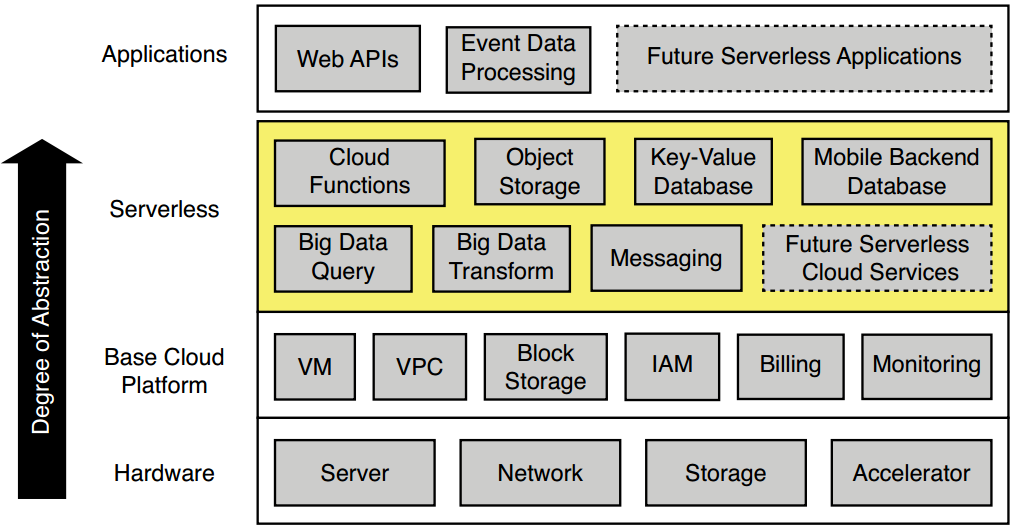
\includegraphics[width=0.8\linewidth]{figs/architecture}
	\caption{Serverless cloud体系结构。serverless层位于应用层和基础云平台之间,简化了云编程。Cloud Functions(例如FaaS)提供了通用的计算并且实现在了专门的BaaS生态(有对象存储,数据库和讯息的服务)中。更具体的,一个在AWS生态中的Serverless应用除了使用Lambda来运行函数外,可能会配套的使用S3(对象存储)和DynamoDB(键值数据库);一个在Google's cloud上的使用Cloud Functions可能配套有Cloud Firestore(移动后端数据库)和Cloud Pub/Sub(讯息)。Serverless还会包含特定的大数据服务如AWS Athena和Google BigQuery,和Google Cloud DataFlow和AWS Glue(大数据传输)。另外在基础平云台上,由供应商提供的有VM,私有网络(VPC,private networks),虚拟化的块存储,用于身份认证的IAM(Identity and Access Management),同时还有后台的计费和事实监测服务。(\cite{jonas2019cloud}图1)}
	\label{figs:architecture1}
\end{figure}
用户只需要编写并上传代码,声明触发事件;Serverless服务供应商就会负责实例出函数执行所需的系统环境来执行该函数,涵盖了实例选择、自动缩放、代码与数据部署、容错、日志、安全补丁和版本更新等脏活累活。

自此,Serverless computing成为了近几年来云计算领域最为火热的概念之一。根据谷歌查询请求的搜索关键词趋势显示,其热度甚至可以和之前如日中天的MapReduce概念的巅峰时期相媲美,如图\ref{figs:trend}所示。
\begin{figure}[!htbp]
	\centering
	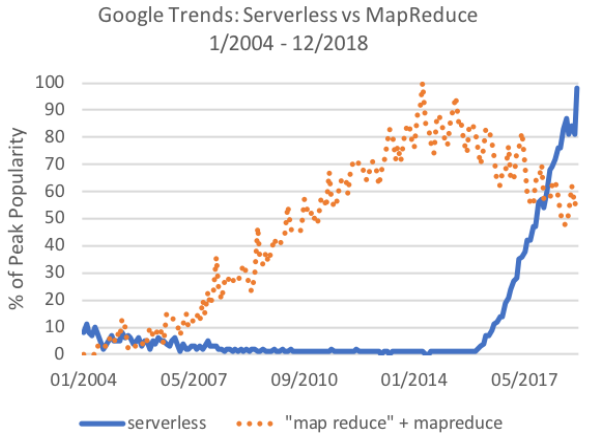
\includegraphics[width=0.5\linewidth]{figs/trend}
	\caption{$ 2014\sim2018 $年谷歌搜索关键词``Serverless''和``MapReduce''的趋势对比。(\cite{hellerstein2018serverless}图1)}
	\label{figs:trend}
\end{figure}
但事实上Serverless computing是一个非常模糊的概念,并没有一个清晰的定义,每个Serverless云平台的供应商(Amazon、Google、Microsoft)都有自己的一套解读并以营销的手段推广之。基本的思路都是:应用开发人员只需要向云平台上传自己的代码(当今的FaaS产品都支持多种语言,例如Python、Java、JavaScript、Go)完成注册函数;声明触发每个功能的事件;接着FaaS架构会监视这些触发事件;由云平台的供应商来管理资源的分配与调度,为用户定义的函数分配运行时(runtime),按需自动缩放(autoscaling)函数执行的运算资源,并将结果持久化\cite{hellerstein2018serverless};而用户仅需要按照函数实际执行时间付费,也即pay-as-you go模式。这样,程序开发者不需关心服务器的配置和运行,可以看做是``Serverless''概念最直观的理解。以AWS Lambda为例,Serverless模式如图\ref{figs:flow}所示。
\begin{figure}[!htbp]
	\centering
	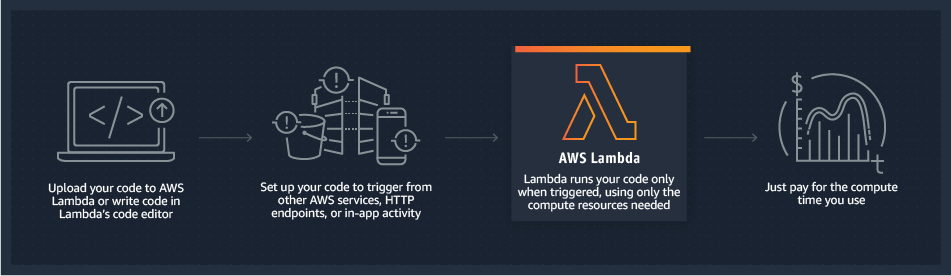
\includegraphics[width=0.7\linewidth]{figs/flow}
	\caption{https://aws.amazon.com/lambda/}
	\label{figs:flow}
\end{figure}

虽然我们不计较Serverless computing的精确概念,但是仍然有必要厘清楚两对容易混淆的技术概念之间的关系。

\textbf{Serverless computing和Lambda/FaaS(Function as a Service)的关系}。Cloud functions被视为属于FaaS范式,也确实被视为Serverless computing的核心理念。但是FaaS本身提供不了什么价值,函数执行短暂而且互相隔离;除了触发以及自动扩展函数执行的机制外,在FaaS上构建应用程序还需要在持久和临时存储中进行数据管理\cite{hellerstein2018serverless}。所以虽然Severless的概念是由Lambda/FaaS兴起的,但是两者并不等同。Serverless不仅仅是FaaS,还需要加上由供应商提供的各式各样多租户自动缩放服务的``标准库''支持;对于AWS来说,这包括S3(大对象存储)、DynamoDB(键值存储)、SQS(排队服务)、SNS(通知服务)等\cite{hellerstein2018serverless}。换言之,云平台为了迎合特定应用的需求,还提供了以BaaS(Backend as a Service,如Serverless数据库、对象存储和大数据处理服务等形式存在的Serverless框架。一种简单的理解是:Serverless Computing = FaaS$ + $BaaS\cite{jonas2019cloud}.

\textbf{Serverless computing和Kubernetes的关系}。Kubernetes作为一种``容器编排''技术是用来部署微服务(microservices)的\cite{jonas2019cloud}。微服务和Serverless computing又有着千丝万缕的关联,但这里我们就不展开讨论了。Kubernetes本质上是一种简化的Serverful computing管理技术。由于多年来Google内部的开发和使用,它得以快速发展。虽然脱胎于Serverful computing,但是Kubernetes可以提供短期的计算环境,和Serverless一拍即合,并在硬件资源、执行时间和网络通信方面有更少的限制。托管的Kubernetes产品有Google Kubernetes Engine(GKE)和AWS Elastic Kubernetes Service(EKS),另外微软的Azure Serverless云系统的实现也是基于Kubernetes。但是托管式的Kubernetes服务和Serverless服务之间有一个关键区别:\textbf{计费模型}——前者按照分配的资源收费,而后者按照函数执行时间,也即真实使用的资源收费\cite{jonas2019cloud}。由此可见,虽说Kubernetes不是为了Serverless专门设计的,但是工业界还是很会普遍的复用Kubernetes,通过在其上进行封装使得Serverful的逻辑对上层用户不可见来实现Serverless computing。

总结一下,Serverless计算和传统的与之对立的Serverful计算有四个关键的不同之处:
\begin{enumerate}
	\item 用户执行代码不需要管理资源分配。而且这些代码大多功能单一,无状态。
	\item Serverless平台责任方根据实际计算的需要,快速地对资源进行自动缩放(autoscaling)。
	\item 计算与存储解耦合。数据存储由另外的云服务来提供服务。因此两者的分配和价位彼此独立。
	\item 以使用的资源付费(如执行时长)而不是分配的资源(如分配的VM的大小和数量)。
\end{enumerate}

\section{Amazon AWS Lambda初探(周盈坤)}\label{sec:lambda}
Amazon的AWS Lambda是第一个提出Serverless服务的云平台。但这个结论并不是没有争议的。一些人可能会指出上世纪90年代流行的共享web主机环境提供了许多Serverless computing范畴的功能;例如它们也有无状态的编程模型、多租户模式、对可变需求的强行响应和一套标准化的函数调用API、公共网关借口(CGI)、甚至允许直接部署用Perl或PHP等高级语言编写的代码\cite{jonas2019cloud}。而作为Amazon EC2的老对手,Google最初的App Engine也允许开发者直接部署代码,同时大部分的操作交由云平台来完成。但是App Engine模式在Severless正在开始流行的这几年之前,基本上不被市场接纳,惨败于EC2模式。所以Lambda既然带火了Serverless,那么它一定有过人之处。它与之前产品的最大不同指出在于提供了真正能够大规模运用的自动缩扩容能力,跟踪应用的负载,快速响应资源需求,如在没有需求的情况下能将资源一直缩减为零;并以一种更加细粒度的方式管理,如最小时长单位为100ms的按时计费服务。
\subsection{The use cases}
百闻不如一见,我们首先来见识几个使用Lambda函数的实际用例。下面给出6个Severless computing的使用案例。为了论述的完整性,这里简单阐述一下用例中使用的backend服务的作用(参考\href{https://aws.amazon.com/serverless/}{AWS Serverless}官网)。
\textbf{Amazon S3(Simple Store Service):}提供安全、持久且高扩展性的对象存储服务,同时易于使用,具有简单的Web服务端口,用于在Web上的任何位置存储和检索任意数量的数据;
\textbf{Amazon Kinesis:}是一种AWS上流式处理数据的平台,可以帮助开发者轻松加载和分析流数据,另外还能让开发者根据具体需求来构建自定义流数据应用程序;
\textbf{Amazon DynamoDB:}快速灵活的NoSQL服务,适合所有需要一致性且延迟低于10毫秒的任意规模的应用程序;
\textbf{Amazon Redshift:}是种快速且完全托管的数据仓库服务,让开发者可以使用标准SQL和现有的商业智能工具经济高效地分析您的所有数据,提供优质的数据仓库解决方案;
\textbf{Amazon API Gateway:}提供完全API托管服务,可以帮助开发者轻松创建、发布、维护、监控和保护任意规模的API,同时可以帮助开发者处理成千上万个并发API调用和流量管理、授权、访问控制、监测以及API版本管理;
\textbf{Amazon SNS:}一种完全托管的发布/订阅消息收发服务,可以轻松分离和扩展微服务、分布式系统和无服务器应用程序。
\begin{enumerate}
	\item 实时文件处理应用。如图\ref{figs:eg3}使用S3来触发AWS Lambda,将Lambda函数对上次的拍摄的照片进行根据桌面手机的不同屏幕大小实时调整图片大小。Lambda函数类似的功能还有实时创建缩略图、转换视频代码、建立文件索引、处理日志、验证内容以及聚合和筛选数据。
	\item 物联网IoT后端应用。如图\ref{figs:eg6}将传感器的数据发送到Kinesis上,接着由Kinesis触发AWS Lambda;Lambda根据规则自动进行订单的组装。
	\item 实时数据流处理应用。如图\ref{figs:eg4}使用Kinesis实时地将社交媒体流数据加载进来,触发AWS Lambda;Lambda运行函数产生哈希标签趋势数据(hashtag trend data);这些数据会存入DynamoDB中,用来提供商业用户对这些社交媒体趋势数据的及时查询。类似的功能还有通过实时流数据跟踪应用程序活动、整理数据、生成指标、帅选日志、建立索引、分析社交媒体以及遥测和计量IoT设备数据。
	\item 数据仓库中的大数据分析应用。如图\ref{figs:eg5}展示了电子商务公司普遍存在的一个应用场景——对用户的购物行为进行分析。线上的订单数据会被存入DynamoDB中;AWS Lambda针对DynamoDB表中每个数据更改执行数据验证、筛选、排序或者其他转换(ETL, database Extract, Transform, and Load);接着将转化后的数据加载到RedShift数据仓库中;最后从数据中自动产生分析。
	\item Web应用程序。这是一类非常流行的应用,用到了如图\ref{figs:eg1}所示的同步调用的模式,其中关键的一点是使用API Gateway。对于这个搜索当地天气信息的App来说,网页前段的代码会从S3中经由用户点击这个时间传送到API Gateway;接着触发AWS Lambda运行代码从DynamoDB中获得天气的信息并且返回数据给用户。
	\item 移动后端应用。如图\ref{figs:eg2}展示了媒体社交平台普遍存在的一个应用场景——用户发布了自己的更新状态,平台App通过API Gateway触发AWS Lambda;Lambda函数会查看用户的朋友列表并且初始化状态更新的通告;接着状态更新通告就会通过SNS服务推送给用户的朋友;这些朋友们就能在自己的移动端接收到状态更新通告了。
\end{enumerate}
%TODO: https://aws.amazon.com/lambda/
\begin{figure}[!htbp]
	\begin{subfigure}[b]{0.49\linewidth}
		\centering
		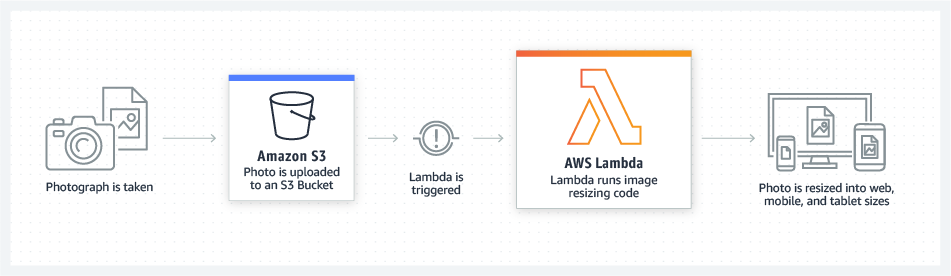
\includegraphics[width=\linewidth]{figs/eg3}
		\caption{}
		\label{figs:eg3}
	\end{subfigure}
	\begin{subfigure}[b]{0.49\linewidth}
		\centering
		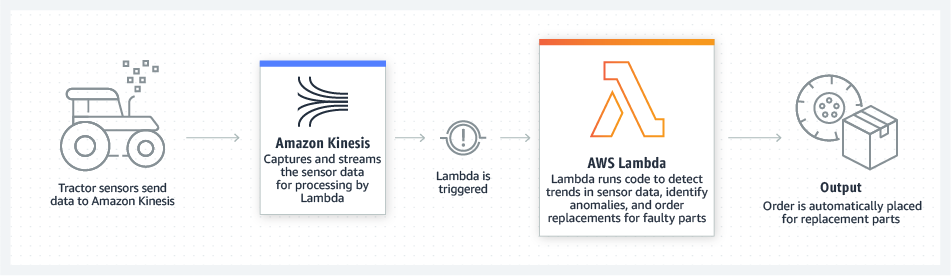
\includegraphics[width=\linewidth]{figs/eg6}
		\caption{}
		\label{figs:eg6}
	\end{subfigure}
	\begin{subfigure}[b]{\linewidth}
		\centering
		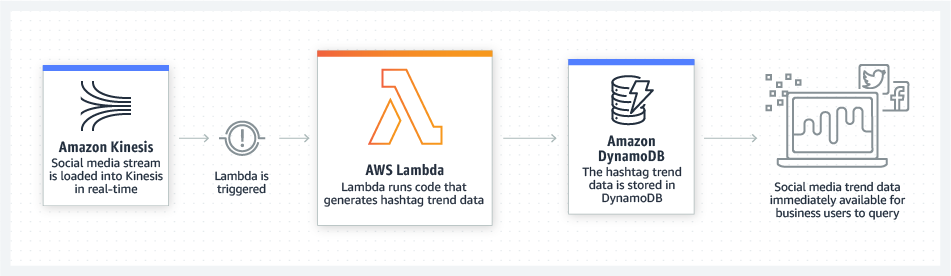
\includegraphics[width=0.8\linewidth]{figs/eg4}
		\caption{}
		\label{figs:eg4}
	\end{subfigure}
	\begin{subfigure}[b]{\linewidth}
		\centering
		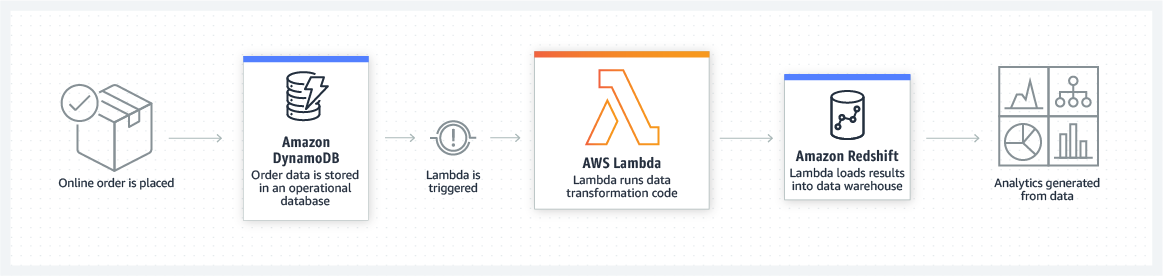
\includegraphics[width=0.8\linewidth]{figs/eg5}
		\caption{}
		\label{figs:eg5}
	\end{subfigure}
	\begin{subfigure}[b]{\linewidth}
		\centering
		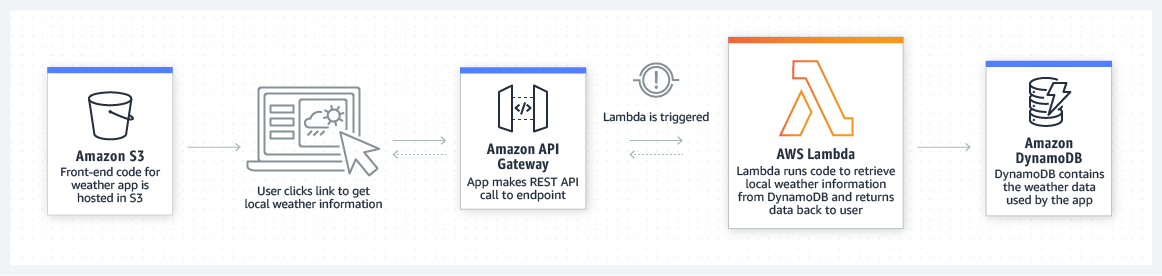
\includegraphics[width=0.8\linewidth]{figs/eg1}
		\caption{}
		\label{figs:eg1}
	\end{subfigure}
	\begin{subfigure}[b]{\linewidth}
	\centering
	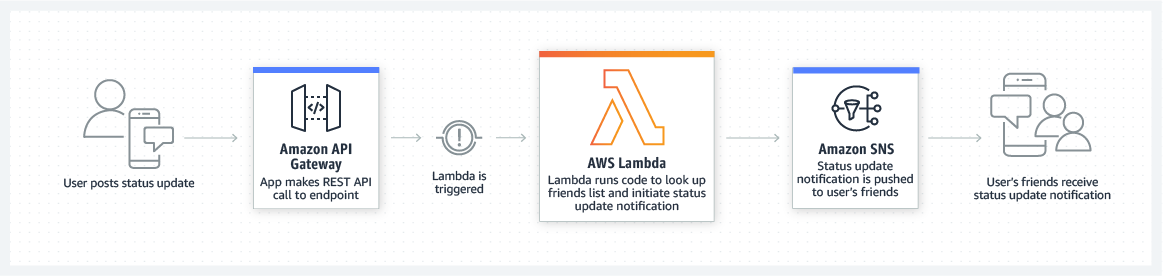
\includegraphics[width=0.8\linewidth]{figs/eg2}
	\caption{}
	\label{figs:eg2}
	\end{subfigure}
	\caption{}
	\label{}
\end{figure}
如下为\cite{serverless}在2018年统计的6大Serverless computing使用最多的应用场景,和上述的6个实际用例相呼应。
\begin{table}[!htbp]
	\caption{}
	\label{tab:usage}
	\centering
	\footnotesize% fontsize
	\setlength{\tabcolsep}{4pt}% column separation
	\renewcommand{\arraystretch}{1.2}%row space 
	\begin{tabular}{ll}
		\hline
		占比 & 用例\\%inserts table 
		\hline
		32\%   & Web and API serving. 如例子\ref{figs:eg1}和\ref{figs:eg2}所示。\\
		21\%   & Data Processing, e.g., batch ETL (database Extract, Transform, and Load). 如例子\ref{figs:eg4}和\ref{figs:eg5}所示。\\
		17\%   & Integrating 3rd Party Services. \\
		16\%   & Internal tooling. 如例子\ref{figs:eg3}所示。\\
		8\%    & Chat bots e.g., Alexa Skills (SDK for Alexa AI Assistant). \\
		6\%    & Internet of Things. 如例子\ref{figs:eg6}所示。\\
		\hline
	\end{tabular}
\end{table}
从具体的实际用例中抽象出来,Lambda函数有三种不同形式的调用方式。分别是同步(Synchronous)调用、异步(Asynchronous)调用和基于轮询(Poll-Based)调用,如图\ref{figs:invoke}所示。同步调用是最直接的一种方式,通过API Gateway来调用的,如例子\ref{figs:eg1}和\ref{figs:eg2}所示。反映在命令行中为:
\begin{lstlisting}[language=bash]
aws lambda invoke —function-name MyLambdaFunction —invocation-type RequestResponse —payload  “[JSON string here]”
\end{lstlisting}
异步调用是事件驱动的。Amazon的S3和SNS等服务都可以产生事件来调用Lambda函数,如例子\ref{figs:eg3}和\ref{figs:eg5}所示。反映在命令行中为:
\begin{lstlisting}[language=bash]
aws lambda invoke —function-name MyLambdaFunction —invocation-type Event —payload  “[JSON string here]”
\end{lstlisting}
基于轮询调用主要是为了实时性的服务而设计的,比如加载流数据的Kinesis和产生流数据的DynamoDB Streams,如例子\ref{figs:eg6}和\ref{figs:eg4}所示。
\begin{figure}[!htbp]
	\centering
	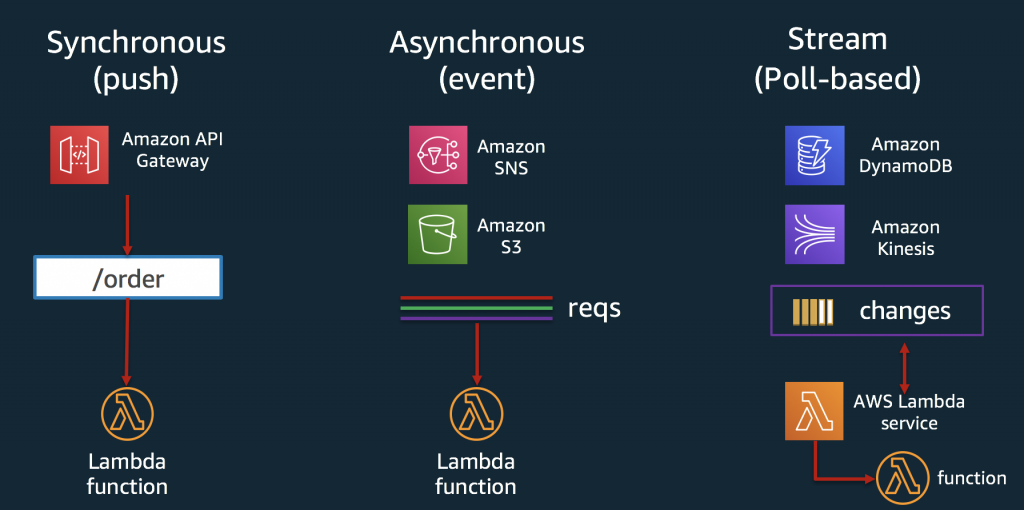
\includegraphics[width=\linewidth]{figs/invoke}
	\caption{https://aws.amazon.com/blogs/architecture/understanding-the-different-ways-to-invoke-lambda-functions/}
	\label{figs:invoke}
\end{figure}

所以从AWS Lambda上,我们可以看到当下的Serverless computing相较之前的产品要成熟得多,得益于背后Amazon强大完整的生态支持(BaaS的思想),得益于更好的自动缩扩容、更安全的隔离性和更灵活的云平台。Serverless computing多采用多租户共享硬件的模式,所以依赖于高性能和隔离安全性。VM或容器提供的隔离是当前cloud function下多租户的事实上的标准。但是因为VM或者容器配置(冷启动)需要很长的时间,为了缩短这个时间,Serverless computing供应商使用复杂的技术来加快函数运行环境的创建。AWS Lambda中使用的方法是维护一个VM实例``热池'',和一个之前执行过的函数实例的``活跃池''以快速响应未来可能到来的调用\cite{jonas2019cloud}。资源的生命周期管理和多租户下的bin packing是Serverless computing中提高资源利用率以及性能的核心技术。所以近几年来的一些工作旨在通过利用Unikernel、Firecracker、gVisor等技术来减少多租户隔离所带来的开销。

\subsection{Serverless computing architecture之AWS Lambda implementation}
在Serverless computing的架构中,还需要考虑的因素的因素有负载平衡、故障处理等。下面我们来介绍Amazon早期对Serverless computing的实现。Lambda早期是将用户函数运行在独占的EC2虚拟机中的Linux容器上的。其架构和软硬件栈如图\ref{figs:arch}所示。Linux容器采用Linux控制组(cgroups)和命名空间(namespace)。其中,cgroups定义进程的使用资源(CPU、内存、网络等);namespace定了一个进程的访问权限(uid,gid,pid,mount,filesystem等)。除了cgroups和namespace,Linux容器还会使用到seccomp技术。seccomp是内核防火墙,限制一个进程对内核系统调用systemcall的访问权限,因此能够在应用程序和内核之间提供更好的隔离。但是它们要求用户创建预定义的系统调用白名单。然而在实际中,很难事先罗列出应用程序所需要的所有系统调用。因此容器之上还需要用沙盒(sandbox)来加固隔离安全性。
\begin{figure}[!htbp]
	\begin{subfigure}[b]{0.49\linewidth}
		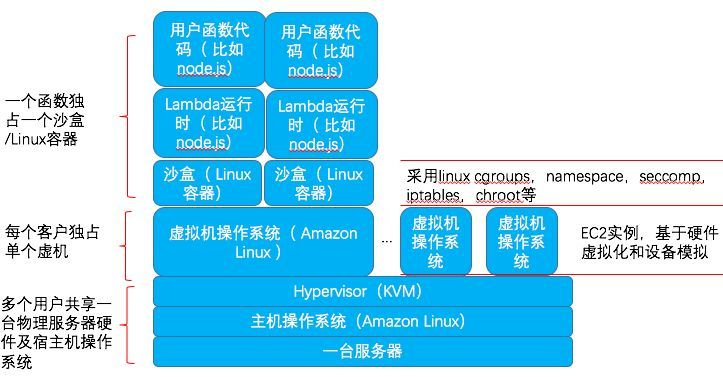
\includegraphics[width=\linewidth,height=0.21\textheight]{figs/arch}
		\caption{}	
	\end{subfigure}
	\begin{subfigure}[b]{0.49\linewidth}
		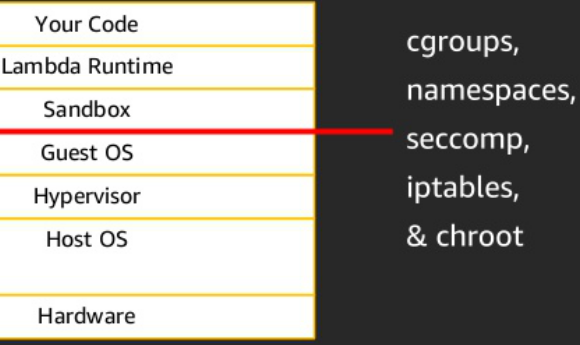
\includegraphics[width=\linewidth]{figs/stack_0}
		\caption{}
		\label{figs:stack_0}
	\end{subfigure}
	\caption{https://cloud.tencent.com/developer/article/1452524}
	\label{figs:arch}
\end{figure}

如图\ref{figs:block}展示了Lambda的技术架构。
\begin{figure}[!htbp]
	\centering
	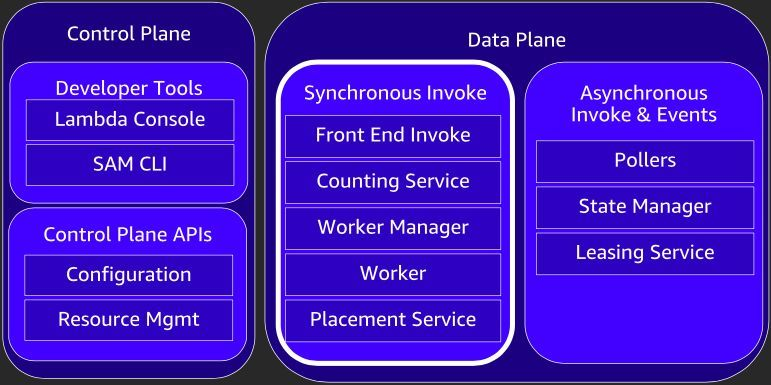
\includegraphics[width=0.6\linewidth]{figs/internal}
	\caption{}
	\label{figs:block}
\end{figure}
这里我们将目光聚焦在中间白色粗边框起来的部分,其中:Front End Invoke能够编排同步调用也能编排异步调用;Counting Service提供了一个用户并发的域范围视角来强制设置限额;Worker Manager追踪容器空闲和忙碌的状态,并且为新来的函数调用请求调度可用的容器;Worker为用户代码提供一个安全的执行环境;Placement Service将沙盒放置在workers上,在不影响用户体验或者冷路径延迟(cold-path latency)的前提下,最大化packing的密度。
具体地,或者更为直观的理解,在早期一个worker就是一个EC2实例,其操作系统为Amazon Linux。图\ref{figs:worker}是worker被创建以及函数被调度到worker中的基本流程。其中,Worker manage负责worker的创建和管理,Placement负责将用户的函数调度到某个或某些worker上运行。流程为:用户请求通过ALB(Application Load Balancer)转发给Front End;接着Front End发送请求至Worker Manager;Worker Manager初始化Worker;Worker准备函数沙盒执行环境;Worker启动后将状态原路返回给Front End;最后交由Front End触发函数执行。
\begin{figure}[!htbp]
	\centering
	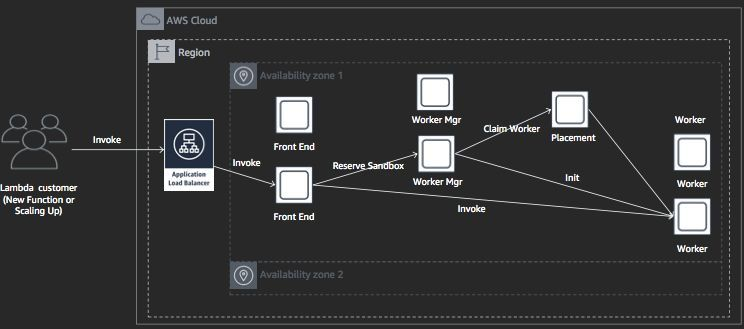
\includegraphics[width=0.8\linewidth]{figs/worker}
	\caption{}
	\label{figs:worker}
\end{figure}
用AWS Lambda软硬件栈的视角来看,如图\ref{figs:stack}所示。用户函数运行在Lambda Runtime中;再下面是沙盒;沙盒的下边界(见图\ref{figs:stack_0})使用了cgroups, namespaces, seccomp, iptables和chroot等结构以实现操作系统层级上的虚拟化;再往下两层是实现安全隔离的关键——虚拟化技术与设备模拟。
\begin{figure}[!htbp]
	\begin{subfigure}[b]{0.49\linewidth}
		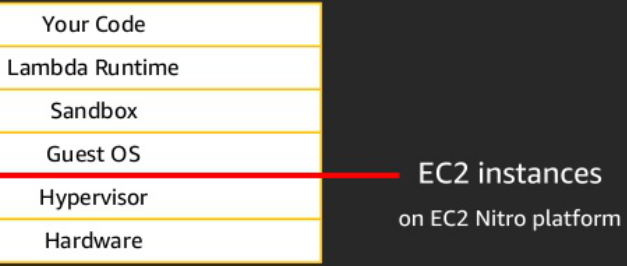
\includegraphics[width=\linewidth]{figs/stack}
		\caption{}
		\label{figs:stack}	
	\end{subfigure}
	\begin{subfigure}[b]{0.49\linewidth}
		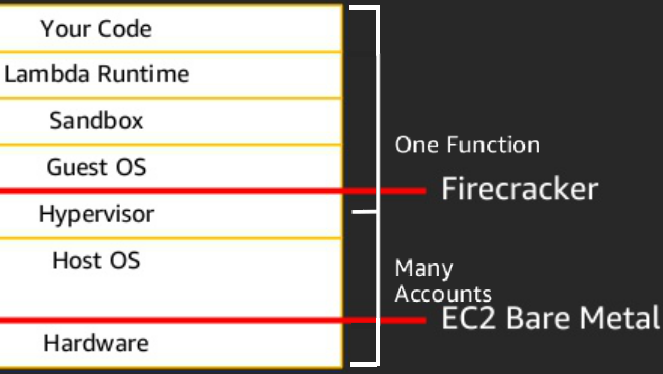
\includegraphics[width=\linewidth]{figs/stack_2}
		\caption{}
		\label{figs:stack_2}
	\end{subfigure}
	\caption{}
\end{figure}
早期的Lambda服务始于EC2实例上构建worker,好处有:1)安全边界清晰,2)快速构建系统并上限业务。但是Amazon后来意识到,基于EC2实例的Lambda存在着明显的缺陷:
\begin{itemize}
	\item 浪费资源:用户一个简单的测试函数也会占用一个EC2虚机。
	\item 启动速度:EC2虚机的创建时间很长。
	\item 管理复杂:需要管理复杂的资源和安全模式。
\end{itemize}
并不适合今天Serverless computing的需求——资源利用率高、启动快、有更好的扩展性同时管理便捷。为了达到以上三点,并且不以损失性能为代价,Amazon决定对早期的Lambda进行改进,在此过程中开发了Firecracker微虚机,如图\ref{figs:stack_2}所示。更深入的介绍参见章节\ref{sec:Firecracker}。接来下的章节\ref{sec:berkeley}我们先来看看来自伯克利分校的学者对于Serverless computing的见解。


%以上,介绍了程序员的视角如何使用AWS Lambda平台。但是我们更好奇的是Lambda是如何实现自动缩扩容、强隔离以及运行环境管理与资源分配的。
\section{Serverless Computing之Berkeley Views(周盈坤)}\label{sec:berkeley}
2018年年底和2019年年初,时隔两个月的时间,加州大学伯克利分校的学者们(出自同一个实验室)发了两篇近几年来在Serverless Computing领域颇有影响力的文章\cite{hellerstein2018serverless,jonas2019cloud}。将这两篇论文对比起来看可以发现:一个唱红脸一个唱白脸。特别有意思。前者\cite{hellerstein2018serverless}唱白脸,负责泼冷水,砸Serverless Computing的场子,犀利的指出第一代Serverless computing的局限性和关键缺陷;后者\cite{jonas2019cloud}唱红脸,负责回顾,总结和展望Serverless Computing,并乐观的认为:实现和完善是一步一步来的,各种工程上的挑战也都是暂时的,Serverless Computing有着光明的未来。我们依次来解读这两篇文章。

\subsection{Serverless Computing: One Step Forward, Two Steps Back}
文章\cite{hellerstein2018serverless}试图提醒人们在跟风追求潮流的时候,应该回归理性,用批判性的思维来审视Serverless computing。这篇文章为了避免泛泛而谈,选择了AWS的FaaS框架的Lambda作为明确的讨论主体。

首先,按照函数的调用交互可以将Serverless use cases划分为3个类别\cite{hellerstein2018serverless}:
\begin{enumerate}
	\item 尴尬的并行函数。每个函数都是独立的任务,不需要和其他函数交互和相互通信。而且要求这些任务能够在短时间内比如几分钟完成。这类应用能够直接利用Lambda自动缩放的特性来按需向上或向下扩展。
	\item 编排函数。利用Serverless函数来完成简单的服务调用编排。例如在Lambda上实现查询服务应用。具体的查询以及数据处理是由Amazon提供的云服务Athena和S3来完成的,Serverless函数在这里值起到一个统筹指挥的作用。
	\item 函数组合。应用是由函数的集合组成的,这些函数串在一起,上一个函数的输出是下一个函数的输入。这些函数通常要操作状态,所以往往和排队系统(比如SQS)或者对象存储(比如S3)
\end{enumerate}
总的来说,Serverless以及目前的FaaS方案对第一中类别的应用场景更具有吸引力,也即简单的、独立的任务,并且相互之间没有通信。而use cases中如果包含了有状态的任务,则就有令人无法接受的高延迟——云供应商宣传的10分钟长周转时间。

下面回到正题:对标题\textit{Serverless Computing: One Step Forward, Two Steps Back}的阐述。自然地,分成了两个方面:
\begin{enumerate}
	\item \textbf{One Step Forward的观点}\begin{quote}
		By providing autoscaling, today's FaaS offerings take a big step forward for cloud programming, offering a pratically manageable, seemingly unlimited compute platform.\cite{hellerstein2018serverless}
	\end{quote}
	Serverless使得能够弹性地、按照需求地使用云资源,是一大进步。
	\item \textbf{Two Steps Back的观点}\begin{quote}
		First, they painfully ignore the importance of efficient data processing. Second, they stymie the development of distributed systems.\cite{hellerstein2018serverless}
	\end{quote}
	两个退步的地方:首先因为每个函数是彼此隔离运行的,而且是无状态的。所以它们之间的交互是通过持久或临时的存储、事件驱动来完成的。这样导致了完成交互的时间比传统架构慢了很多;其次通常分布式系统会依赖如Leader选举、数据一致性和事务提交的技术机制,而这些在目前的FaaS平台上是很难去实现的。
\end{enumerate}
比起One Step Forward进步方面,从篇幅上来看,作者显然是想强调Two Steps Back退步方面。在进步方面,文章花费的笔墨很少,只提到各大供应商都宣传的三大关键特性:1)无限的数据存储,无限的分布式计算能力,以及按照使用的资源付费,而不是以所需要资源的峰值持续付费。接下来的大段篇幅都是在揭Serverless computing的短处。首先是Severless的局限性,以AWS Lambda为例,陈列了如下四点\cite{hellerstein2018serverless}:
\begin{enumerate}
	\item \textbf{受限的存活时间}\ \ 函数调用如果超过15分钟,会被Lambda停止。虽说Lambda可能会将函数的状态缓存入当前运行的主VM(Virtual Machine虚拟机)上,来支持热启动。但是没有机制能够保证下次执行该函数是在同一个VM上。
	\item \textbf{I/O瓶颈}\ \ 目前FaaS通过网络借口的方式来连接云服务,尤其是共享存储。网络限制了I/O吞吐量。最近的研究表明单个Lambda函数的平均网络带宽是538Mbps,当然了,Google和Azure也是半斤八两,比单个现代SSD慢了一个数量级。更糟糕的是,在一个VM上往往有多个函数共享带宽——假设有20个,那么每个函数的平均带宽只有可怜的28.7Mbps.
	\item \textbf{通过低速存储进行通信}\ \ Lambda函数在运行时不能以任何方式直接进行网络寻址。结果是,两个Lambda函数只能通过自动缩放的中间服务(比如S3)进行通信;这意味着像S3存储系统比点对点的网络速度更慢,成本更高。跨客户端调用维护状态需要将状态写入慢速存储,并在每次后续调用时将其读出。而这个读写状态的延迟高的可怕。例如,在处理客户端请求时,每个函数被分配到流程中的一个子任务。每个子任务都应该知道当前请求的上下文,也就需要保存会话状态。但是Serverless的无状态特性使得每个子任务的会话信息不能直接共享,需要像保存到慢速的存储服务如S3中,然后下游的子任务在从S3中获取上下文,接着执行。
	\item \textbf{无专用硬件}\ \ FaaS/Lambda目前只支持设置CPU超线程的时间片和内存使用量,而对GPU等专用硬件的支持不够——没有API或其他机制来访问这些加速专用硬件。
\end{enumerate}

上述的局限性会直接推导出如下的问题\cite{hellerstein2018serverless}:
\begin{enumerate}
	\item \textbf{FaaS是Data-shipping架构}\ \ 这可能是FaaS平台和其APIs最大的架构缺陷。Serverless函数运行在隔离的VM上,与数据分离。此外,Serverless函数是短暂存在的其不可寻址的,因此它们在内部缓存状态以服务重复请求的能力是有限的。所以FaaS通常是``将数据传送到代码(shipping data to code)'',而不是``将代码传送到数据(sihpping code to data)''。但是存储器层次结构的实际情况——跨越各种存储层和网络延迟——由于延迟、带宽和成本的原因,使得data-shipping是一个糟糕的设计。
	\item \textbf{FaaS阻碍了分布式计算的发展}\ \ 由于Serverless函数没有网络可寻址性,因此只有通过缓慢而昂贵的存储传递数据,两个函数才能以Serverless的方式系统工作。这阻碍了基于细粒度通信协议如leader选举、成员资格、数据一致性和数据提交。很多分布式和并行应用程序——尤其是科学计算——也依赖于细粒度的通信。尽管另一种看法是FaaS鼓励基于全局状态的新的事件驱动的分布式编程模型。但是事件处理仍然需要将全局状态的部分从慢速存储传递到Serverless函数。同时,当前的Serverless存储在副本之间提供了弱一致性。
	\item \textbf{FaaS阻碍了有硬件加速的软件创新}\ \ 当前的FaaS产品都运行在统一且相当平凡的VM平台上,没有提供GPU等用户自定义的硬件加速的软件执行机制。但是可喜的是,中国的企业如华为云平台已经提供了GPU加速的支持,可以参见网址\url{https://www.huaweicloud.com/product/cci.html}. 此外FaaS平台也无法支持内存数据库系统——最大的Lambda实例也只被允许最大3GB的RAM。缺乏对这些硬件的访问以及适当的定价模型,显著限制了FaaS产品作为软件创新平台的效用。
	\item \textbf{FaaS不鼓励开源服务的创新}\ \ 流行的开源软件基本上都是有状态的,所以不能在当前Serverless架构中大规模运行。特别是近年来快速增长和成熟的领域——开源数据库系统,将无法在当前的FaaS平台上进行构建。并且,当前Serverless基础架构有意或无意地将用户锁定在平台供应商提供的服务器上。
\end{enumerate}

为了真实的评估这些问题的严重性,文章\cite{hellerstein2018serverless}研究了三个从大数据到分布式计算设置的实例,分别是1)模型训练、2)低时延的预测服务、3)分布式计算。这三个的配置参数比较复杂,具体可以参见原文,这里我们就简单来说:
\begin{enumerate}
	\item \textbf{模型训练}\ \ 使用Lambda函数和EC2实例(instance)来训练相同的任务。对于Lambda来说,数据是存储在S3上的;EC2的数据可以直接存储在云存储EBS上。对这两个方案实测的结果为:1)Lambda:一次迭代训练用了3.08s,其中用户从S3获取100M数据占了2.49s,另外0.59s用来执行迭代优化。运行了31次Lambda函数,每次15分钟,一共用了465分钟花费了0.29美元;2)EC2:一次迭代训练用了0.14s,其中从EBS获得同样大小的数据占了0.04s,另外0.01s迭代优化,一共运行了22分钟,花费了0.04美元。
	\item \textbf{低时延的预测服务}\ \ 这是用已经训练好的模型用来做实时输入的推断预测服务。还是用EC2与Lambda进行对比。其中Lambda平均每个batch最小延时447ms,平均花费\$1584/h;EC2最小延时2.8ms比Lambda快127倍,平均花费为\$27.84/h,比lambda便宜57倍。
	\item \textbf{分布式计算}\ \ 图\ref{figs:latency}展示了6种不同的两个函数或者实例之间传输1KB信息的延时对比,以EC2 NW(network)的实际延时作为归一化系数。由于Lambda I/O(S3)和EC2 I/O(S3),以及Lambda I/O(DynamoDB)和EC2 I/O(DynamoDB)的延时几乎没有区别,而直接使用网络通信的EC2 NW延时低了一到两个数量级。所以基本可以断言,主要的之言是由中间的存储服务造成的。但是上文也已经提到,Lambda的函数之间不能直接通信(因为网络不可寻址),需要借助中介的存储服务如S3、DynamoDB、SQS和SNS来进行间接通信。这是一个致命的缺陷。
	\begin{figure}[!htbp]
		\centering
		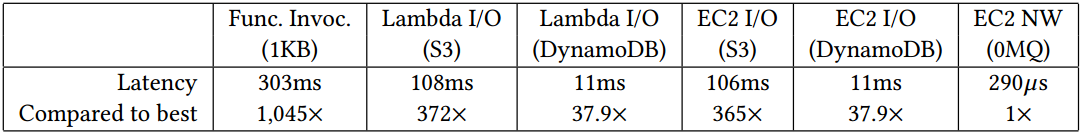
\includegraphics[width=0.7\linewidth]{figs/latency}
		\caption{将不同方式``通信''1KB的延时。为了刻画纯函数化的事件驱动通信,展示了在1KB的参数上调用一个空操作(no-op)Lambda函数,重复1000次取平均时延;接着展示了两个显式的从Python Lambda函数和EC2实例到S3和DynamoDB上的1KB I/Os (write+read)操作,重复5000次取平均时延;最后展示了直接用网络进行1KB的消息传递,使用Python和ZeroMQ消息库运行在两端的EC2实例上运行来测量出来的时延,重复10000次取平均时延。(\cite{hellerstein2018serverless}表1)}
		\label{figs:latency}
	\end{figure}
\end{enumerate}

所以针对目前基于FaaS的Serverless Computing的局限性和体现的问题,文章\cite{hellerstein2018serverless}放眼未来,提出了6点关键而明确的挑战:
\begin{enumerate}
	\item \textbf{流动的代码和数据放置}\ \ 弹性要求代码和数据在逻辑上分离,但是为了获得良好的性能,Serverless架构应该能够并且愿意物理的共享某些代码和数据。所以最好是将代码传动到数据,而不是将数据提取到代码的当前的FaaS普遍做法。
	\item \textbf{异构硬件的支持}\ \ 允许开发人员通过规范将代码定位到特定硬件特征可能是有用的,以促进软硬件协同设计。但是对异构硬件的支持并不意味着就是提倡硬件和服务紧耦合。Serverless平台应该根据程序员提供的或从代码中提取的逻辑性能要求规范,对区分资源的代码分配做出动态的决策。然后可以将这些规范用于更一般的异构性感知来进行资源的时空复用\cite{tumanov2016tetrisched}。
	\item \textbf{长期运行,可寻址的虚拟代理}\ \ 因为FaaS中的函数不具有数据的亲和性,并且没有网络可寻址性,所以重复的请求无法充分利用先前的缓存数据。这样,最好能偶股提供一个长期运行住手在平台上的虚拟代理,而且这个代理是可寻址的。用它来指导函数在哪个具体的VM上运行,以在重复的请求中利用好缓存,来减少数据的传输。
	\item \textbf{无序编程模式}\ \ 如果要真正做到分布式计算时对资源的大小进行自动弹性的调整,更本质的是在编程的模式有所突破,这便是无序的,或者说异步的模式(不同于冯诺依曼体系结构)。
	\item \textbf{灵活编程模式和通用的中间表示层}\ \ 对每个语言来说,实现一整套相关优化是繁重的。所以就非常有必要提供一种用于云端的通用的中间表示层,任何高级语言都可以将代码编译成这个中间层,从而能够统一实现对上文提到的流动的代码和数据放置、异构硬件和无序编程模式这三个挑战的优化和支持。
	\item \textbf{安全性考虑}\ \ 颇为矛盾的是,如果上述的几个挑战在未来都能够得到很好的解决,就会使得Serverless的运维责任方(一般来说也是Serverless平台的供应商)更难以提供安全性的保障。例如允许代码流向共享数据会加剧与多租户机制相关的安全管理挑战以及恶意代码在客户之间利用侧信道攻击收集机密信息的可能性。但是好的一方面是,在安全性上的创新会给新的研究带来机遇——学术圈又有新的工作可做了。
\end{enumerate}

\cite{hellerstein2018serverless}的作者Hellerstein给我的印象确实是这般观点犀利的。我在2018年在加州大学伯克利分校访学的时候,非常凑巧地上过他给本科生教授的数据库系统的课程。

\subsection{Cloud Programming Simplified:
A Berkeley View on Serverless Computing}
文章\cite{jonas2019cloud}论述的套路类似,通过实例应用来暴露出当前Serverless computing平台的局限性,借此提出改进这些局限性的挑战。

这里选择了5个研究项目。1)ExCamera:旨在为向YouTube等网站上传视频的用户提供实时编码服务;2)MapReduce:大数据分析框架,也包括其开源实现的Hadoop和Spark\cite{jonas2019cloud};3)Numpywren:大规模的线性代数计算;4)Cirrus:机器学习训练;5)Serverless SQLite:数据库服务。因为它们本来都是基于传统Serverful云计算的应用,所以文章的研究团队尝试着使用cloud functions来将这些应用改写成serverless版本。而那些阻碍改造的难点就非常自然的凸显出来了。不难返现,除了最后一个Serverless数据库外,前四个项目改造为Serverless computing模式的动机都非常的类似。那就是在这些应用整个计算的过程中,对资源的需求量波动都很大。如:ExCamera的计算量取决于视频文件的大小,从几MB到几GB不等;MapReduce处理有些任务的数据集大小变化会非常明显;Numpywren这类的科学计算量波动;机器学习中有若干步骤,比如预处理、模型训练和超参调整,不同步骤需要的计算资源量也存在这显著的差别。所以如果使用固定数量的集群会造成计算的缓慢(机器数量太少)或者资源的浪费(机器数量太多)。利用serverless计算的弹性缩放扩容能力可以很好的平衡计算速度和资源利用率,同时还可以把科研人员,特别是没有体系结构只是背景的开发者从管理集群的繁琐任务中释放出来。最后的成本-性能结果为:ExCamera性能比VM实例提高了60倍,价格却便宜了6倍;MapReduce排序100TB数据仅比VM实例快了1\%,但多出了15\%的成本;Numpywren完成时间慢了3倍,不过CPU资源的消耗量低了1.26到2.5倍;Cirrus比VM实例快了3到5倍,但是开销也高出了7倍;Serverless SQLite如果仅用cloud functions的FaaS形式实现非常糟糕,因为这些函数独立运行,不能共享内存,而且也无法网络直接寻址,需要利用一些远程持久性存储,这会带来较大的延迟(这一点已在文章\cite{hellerstein2018serverless}的解读中反复出现)。所以数据库的一个合理的做法是依然保留为BaaS的形式。

从实际的用例选择与分析上不难发现,文章\cite{jonas2019cloud}比\cite{hellerstein2018serverless}要乐观很多,或者说要中立客观一些。文章\cite{hellerstein2018serverless}所选择的3个实例传统的云计算无论是性能还是成本大获全胜,这样的分析不免就显得有些偏颇,而有失客观,有刻意迎合自身论证的嫌疑。事实上,Serverless computing后于传统的Serverful云计算提出,又在短时间内获得了大量的关注、讨论和应用,说明它肯定是有自己的过程之处与合理的地方。这在ExCamera的用例中,我们就能看的非常清楚,成本和性能全面提升。这种简单的应用就非常适合Serverless computing。除了Serverless数据库外,另外的3个在两个模式中各有千秋。Serverless方案要么性能高,但是成本也高;要么资源利用率高,但是性能低。只有了数据库这种传统的分布式系统让Serverless模式颇为难堪。接下来是文章\cite{jonas2019cloud}列举的这些应用切换到Serverless模式尴尬的局限之处,和\cite{hellerstein2018serverless}有重合之处,但是态度要温和很多。
\begin{enumerate}
	\item Serverless平台的无状态特性使得很难支持具有细粒度状态共享需求的应用程序,这主要是由云供应商提供的现有的存储服务所限制的。如AWS S3、Azure Blob Storage和Google云存储之类的对象存储服务都具有很高的可伸缩性,并且有廉价的存储成本;但是具有较高的访问成本和延时。而如键值数据库如AWS DynamoDB虽然需要长时间进行扩容,而且存储价格相对高昂,但是访问延迟小。
	\item 接下来的两点在上文的\cite{hellerstein2018serverless}解析中均有提到,反映了Serverless在分布式系统中的弱势。首先Serverless缺乏细粒度的协调机制;其次,Serverless在标准通信模式中性能表现的很差劲。在分布式系统中,广播、聚合和shuffle是非常常见的3种通信原语。这些操作也被经常用于机器学习训练和大数据分析所使用。图\ref{figs:pattern}展示了基于VM和Serverless函数的这3个通信模式的异同点。不难看出基于VM的方案需要远程发送的消息数量比基于Serverless cloud functions的方案大大减少了。这是因为在同一个VM实例上运行的若干任务可以共享数据广播的副本,或者在将部分结果发送到其他实例之间先执行本地聚合。但是因为应用程序无法控制cloud functions的位置(也即位于哪个VM中),就所以无法像VM一样利用好局部性,尤其是shuffle的复杂度大大提高了。
	\begin{figure}[!htbp]
		\centering
		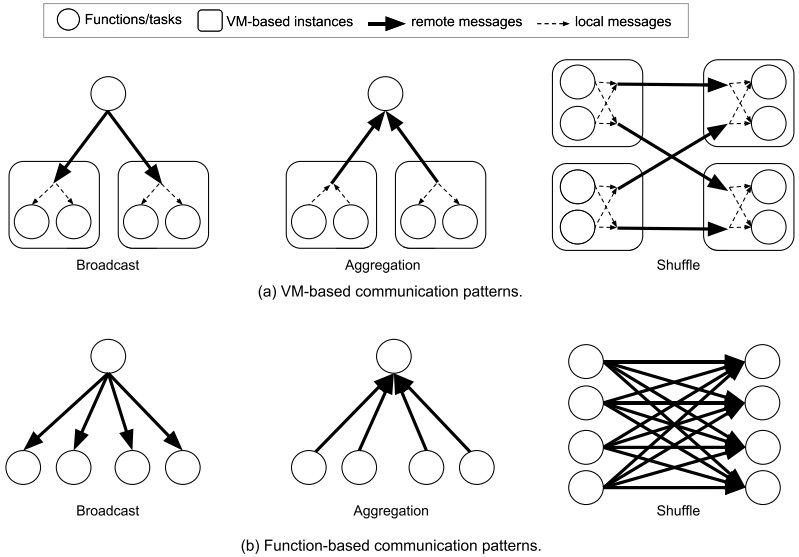
\includegraphics[width=0.6\linewidth]{figs/pattern}
		\caption{通信模式从左到右依次为广播、聚合、shuffle。(a)展示了VM实例上的运行情况;(b)展示了cloud functions实例上的运行情况。}
		\label{figs:pattern}
	\end{figure}
	\item 性能的不可预测性。正所谓成也萧何败萧何,函数运行环境有第三方管理大大简化了程序员的工作,但是也会带来性能的不确定性,比如分配到了不同的硬件资源。其中最突出的问题是冷启动,有三个影响因素:1)启动cloud functions所需要的时间;2)初始化函数的软件环境所需要的时间,如加载Python库;3)用户代码中特定应用程序的初始化。后两个因素往往占主要部分——启动一个cloud functions可能需要不到1秒,但加载所有应用程序库可能需要几十秒。简单的Serverless函数本身运行也不过最多几分钟到十几分钟罢了。
\end{enumerate}

同样的,文章\cite{jonas2019cloud}也提出了Serverless领域未来发展需要解决的挑战,系统地考察了五个领域:
\begin{enumerate}
	\item \textbf{抽象}\ \ 对资源的控制权重口难调,特别是硬件加速器的流行。目前的Serverless抽象阻碍了用户获得对加速器更多的控制权。所以需要提高抽象层次,可以让云供应商推断资源需求,而不是让开发人员执行它们。可以采用的方法有多种,如从静态代码分析以前的运行情况,接着动态重新编译,将代码重定向到其他体系结构。另外Serverless computing的低效的通信模式也是一直所诟病的,如MapReduce和numpywren用例所示。一个解决方案是云供应商公开一个API允许(可选)应用程序指定其计算图谱,从而实现更好的代码数据部署决策,最小化通信开销以提高性能。\cite{jonas2019cloud}的研究团队已经注意到许多通用的分布式框架(如MapReduce、Apache Spark和Apache Beam/Cloud Dataflow)、并行SQL引擎(如BigQuery、Azure Cosmos DB)以及编排架构(如Apache Airflow)其实已经在内部生成了这样的计算图谱。所以原则上,很方便的就能够做到Serverless平台的移植,并通过API将云供应商提供运行的计算图谱。
	\item \textbf{系统}\ \ 这一领域是旨在解决存储和冷启动问题。存储不仅要考虑延时、价格,容错也是必须考虑的。另外,存储还分为临时性存储和持久性存储。而面对冷启动,核心的思想在于尽可能缩减启动量以及提前缓存或者预取。
	\item \textbf{网络}\ \ 和抽象领域中的通信模式重合,最好的解决方案也是让应用程序提供一个计算图谱,使云供应商能偶定位cloud functions,以最小化通信开销。
	\item \textbf{安全}\ \ 这个之前的文章\cite{hellerstein2018serverless}中就有提到,但是并未给出具体的解决之道。Serverless computing重新划分了安全职责,将其中的大部分从云用户转移到了云供应商。然而,Serverless computing还必须解决应用分解后多租户资源共享所固有的风险。物理共享存储是在云平台内部引发硬件级别侧信道攻击和Rowhammer攻击的主要原因。此类攻击首先会寻找和攻击目标位于同一物理主机上的租户作为入侵对象。不过cloud functions的生命周期比较短,且调度存在随机性,会是攻击者难以找到和侵入对象。所以使用一种随机化的、能感知入侵的调度算法将会大大降低此类攻击发生的可能性。但是这样产生的物理隔离有可能会导致启动时间增加、资源利用率降低以及低效通信等问题再次涌现。另外,云函数需要细粒度的安全环境配置,包括获得私钥、存储对象等,并为cloud functions提供易表达的安全接口。值得警惕的是,cloud functions是一把双刃剑,它会通过通信泄露其访问模式和时间信息。而且云函数因为短暂且广泛地分布在整个云上,即便是进行了端到端加密,也有泄露的分解。二阶将Serverless应用分解为许多功能单一的小函数的趋势加剧了这种安全性风险。不幸的是,已有的方法如oblivious算法的开销往往很高。
	\item \textbf{体系结构}\ \ 说到底就是目前对异构硬件的支持不够,其中的观点和\cite{hellerstein2018serverless}类似。
\end{enumerate}

虽然两篇文章论述的套路相似,但是文作者Jonas对Serverless computing表现出来的态度却要乐观很多。他认为上述讨论的Serverless computing的局限性和挑战终将会被克服。困哪只是暂时的,Serverless computing会成为未来云计算的门面\cite{jonas2019cloud}。同时,他的研究团队更是盛赞Serverless computing的出现代表了类似于从汇编语言到高级语言的转变\cite{jonas2019cloud}。这个类比不无道理:高级语言将程序员从寄存器分配和内存管理的繁杂任务中解放出来,提高了逻辑的抽象层次,从而提高了程序员的编程效率;类似的,Serverless computing将程序员从云端的虚拟资源分配和服务器运维的复杂任务中解放出来,使得程序员更加集中精力于业务自身逻辑的应用开发,从而提高开发效率。
%TODO:一个有意思的哲学思辨
%TODO:Google和Azure提供的Severless相差不大。

\section{Amazon AWS Lambda深入---Firecracker(周盈坤)}\label{sec:Firecracker}
%TODO: 强调一下light-weight virtualization technologies
在章节\ref{sec:lambda}中,我们介绍了Lambda早期搭建在EC2虚拟机实例上的Linux容器的组织与管理。并在章节\ref{sec:lambda}的最后提及由于其明显的局限性,Amazon在2018年re:invent大会上宣布开源了一个新的项目工程:Firecracker微虚机(microVM),并已经应用在了Lambda服务之中。

\subsection{概念梳理}
Firecracker与先前的Linux容器方案是有区别的,但是这种区别在认知中容易混淆。这里我们不妨先来厘清楚各种技术之间错综复杂的概念之间的关系。

首先,现在普遍采用的隔离(isolation)技术有三种,分别是\cite{agache2020firecracker}:
\begin{enumerate}
	\item Linux容器,见图\ref{figs:isolation}最右子图;应用运行在容器中,不同的容器按照应用需求配置有不同的库;若干个容器运行在主操作系统内核上。LXC和Docker属于此类。另外,Google为了进一步解决容器的安全性和兼容性的的tradeoff,推出的gVisor也是容器中的一个具体实现。
	\item 虚拟化,见图\ref{figs:isolation}中间子图;应用程序运行在VM中,不同VM按照应用需求配置有不同的库;VM可以看做是Guest OS运行在Hypervisor层上。KVM、QEMU和Unikernel(为了解决冷启动高时间开销等问题)属于此类。另外,本章的主角Firecracker采用的正是此类方案。Firecracker基于KVM,但用更安全的编程语言Rust以及更少的代码(more code$ = $more bug)来替换QEMU。值得一提的是Firecracker包含大约5万行Rust代码,仅是QEMU代码量的4\%.
	\item 语言专用隔离(Language-Specific Isolation)。这一类隔离技术并未在图\ref{figs:isolation}中体现,但是读者一定不会陌生,因为Java虚拟机(JVM)就属于此类。
\end{enumerate}
\begin{figure}[!htbp]
	\centering
	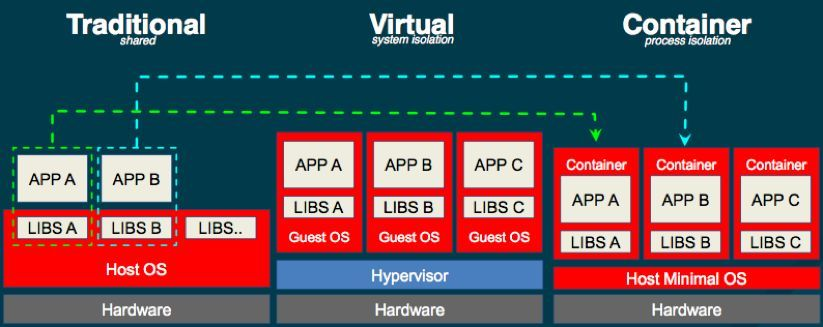
\includegraphics[width=0.8\linewidth]{figs/isolation}
	\caption{从左到右依次为传统的应用进程共享内核结构(无法隔离)、虚拟化技术(应用运行在虚拟机上VM \& GuestOS,提供系统级别隔离)、容器技术(提供进程级别隔离)}
	\label{figs:isolation}
\end{figure}
光有隔离还不够,文章\cite{hellerstein2018serverless,jonas2019cloud}无一不在强调云平台上安全性的重要。为此我们可以在上述的隔离方案中嵌入沙盒(sandbox)机制来增强安全性,如图\ref{figs:sandbox}所示。沙盒对于\ref{figs:sandbox}(a)的Linux容器方案几乎是必选项,因为容器的安全隔离性不够强,需要沙盒加固;而对于\ref{figs:sandbox}(b)的虚拟化技术就是可选项了,因为VMM会内置安全隔离性。
\begin{figure}[!htbp]
	\centering
	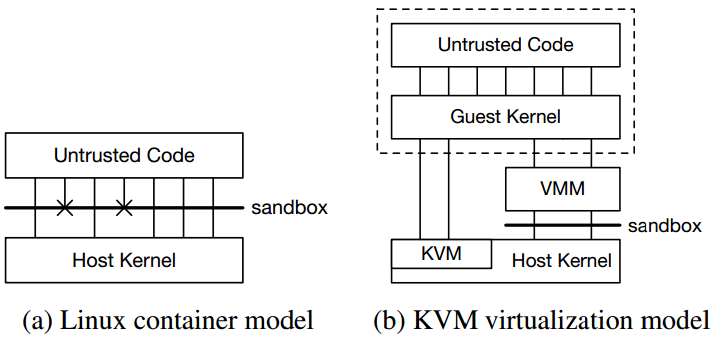
\includegraphics[width=0.5\linewidth]{figs/sandbox}
	\caption{(a)Linux容器的安全模型,直接依赖于内核沙盒的防御攻击能力;(b)KVM虚拟化的安全模型,依赖于Virtual Machine Monitor(VMM)的安全性,可配上沙盒来加固。(\cite{agache2020firecracker}图1)}
	\label{figs:sandbox}
\end{figure}
有了这些基础的背景知识,这里再次强调几点。首先,容器并不是一种虚拟化技术,而是一种进程隔离技术,从内核空间、资源和安全等方面对进程做隔离。其次,Firecracker基于虚拟化技术,因此不属于Linux容器的类别,所以和Google推出的gVisor有着本质的不同。最后,Firecracker不是一种新型的虚拟化技术,依然依赖Intel VT-x,只不过它做的比QEMU精简很多,目的就是完全取代QEMU。那么为什么要取代QEMU呢?原因有很多,例如:庞大的代码体积,其中很大一部分是对基本上用不到的传统设备、总线、机器模型的模拟。虽然能够对各种硬件协议做到真实模拟,一般来讲确实多多益善,但是近年来因为庞大的代码量而高发的漏洞数量,以及针对Serverless computing这样的场景,需要业务启动快、密度高、可快速自动缩扩容,就迫切需要像Firecracker这样提供更为敏捷的运行环境。另外,我们这里不提及Firecracker和Kata Container(有Intel、Hyper.sh和OpenStack主导)的差异。回到主角Firecracker的讨论。

\subsection{Firecracker implementation}
Firecracker像QEMU一样负责创建和管理微虚机。它提高了资源的利用率和计算效率,而且内存开销极低,使得在一台物理服务器上可以常见数千个微虚机。相比之间的Linux容器方案,简单陈列一下其好处有:利用CPU硬件虚拟化实现了用户之间的强隔离性;简化但增强了安全模型;简化了Lambda编程模型;提高了资源利用率;缩短了函数的启动时间。不像Kubernetes,Firecracker就是专门针对Serverless场景设计的,非常适合运行暂时性(transient and short-lived)进程。因为Firecracker是开源的,其网址为\url{https://firecracker-microvm.github.io/},所以有大量公开的信息和设计文档文章可供查阅,还可以直接阅读\href{https://github.com/firecracker-microvm/firecracker}{Github}上的源码。

结合公开的资料,首先我们能够分析出大致几点Firecracker的设计思路与原则。1)内置安全性,支持多租户工作负载的同时做到计算安全性屏障不会被用户有意或者无意的禁用;用户工作负载被认为既神圣不可侵犯的,但又是邪恶的,需要时刻提防。2)轻量虚拟化,重视短暂运行和无状态的工作负载,而非长时间运行和共享状态的工作负载;Firecracker的硬件资源开销是明确且有保障的。3)函数极简,不够构造AWS任务没有明确要求的函数,且每个函数代表的任务功能单一。4)资源的分时复用,Firecracker向用户开放的所有硬件计算资源都可以高效安全地复用。下面我们接着来看Firecracker VMM的特征和体系结构。图\ref{figs:Firecracker}展示的就是Firecracker一个比较完整的体系结构图景。其中,图\ref{figs:host}展示了一个在主机(host)上运行$ n $个Firecracker微虚机的例子:Firecracker运行在Linux的guest OS上(图中显示为Guest的绿色方框);这些guest OS运行在4.14或者更高版本的Linux主机上;蓝色方框和线条是模拟的网络设备;黄色方框和线条是模拟的块存储设备。图\ref{figs:internal}更进一步展示了Firecracker微虚机内部的结构:每个Firecracker进程封装有且仅有一个微虚机。进程里一共运行3种线程:API、VMM和vCPU。
\begin{enumerate}
	\item API线程负责Firecracker的API服务和相关的控制面板,以Unix domain socket的方式向主机提供了一个RESTful API格式的API接口端点。通过这个端点可以对微虚机进行管理和控制,包括:规格配置(如vCPU的个数,用户内存大小)、网络配置(添加网卡)、存储配置(添加虚拟盘,一种基于文件的块设备)、QoS(通过带宽限制和IOPS限制进行流控)、日志配置、启动配置(内核及其参数,根文件系统)、关闭微虚机。
	\item VMM线程向Guest OS暴露出了机器模型、最小化的老式设备模型、微虚机元数据服务(microVM metadata service, MMDS)和VirtIO虚拟网络设备和块设备(用以提供给Guest网络和存储访问服务),并配有I/O速率限制(支持用户按照自己的需求定义灵活的带宽和突发传送的限额)。VMM采用单线程时间驱动模型,对各种I/O请求进行服务。
	\item 除此之外,有一个或多个vCPU线程(每个guest CPU core各一个);它们通过KVM被创造出来,并且运行在\texttt{KVM\_RUN}主循环中;它们在设备模型中执行同步I/O和内存映射I/O操作。
\end{enumerate}
\begin{figure}[H]
	\begin{subfigure}[a]{0.49\linewidth}
		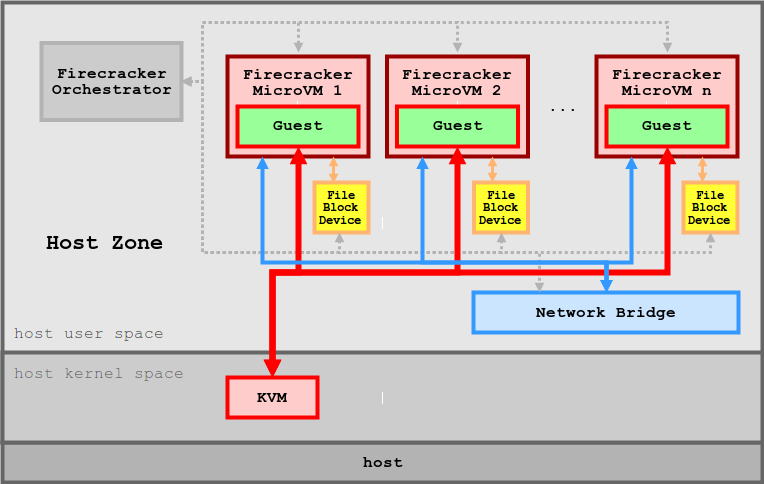
\includegraphics[width=\linewidth,height=0.27\textheight]{figs/firecracker_host_integration}
		\caption{}
		\label{figs:host}
	\end{subfigure}
	\begin{subfigure}[a]{0.49\linewidth}
		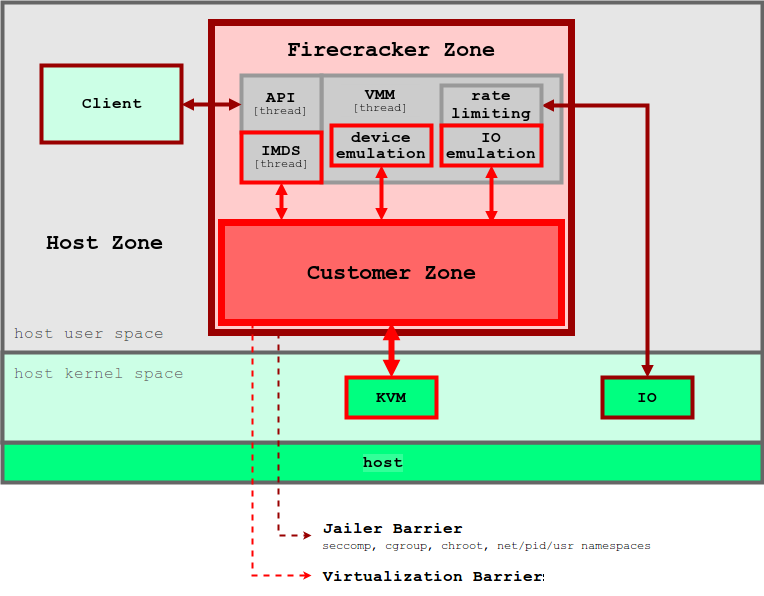
\includegraphics[width=\linewidth]{figs/firecracker_threat_containment}
		\caption{}
		\label{figs:internal}
	\end{subfigure}
	\begin{subfigure}[b]{\linewidth}
		\centering
		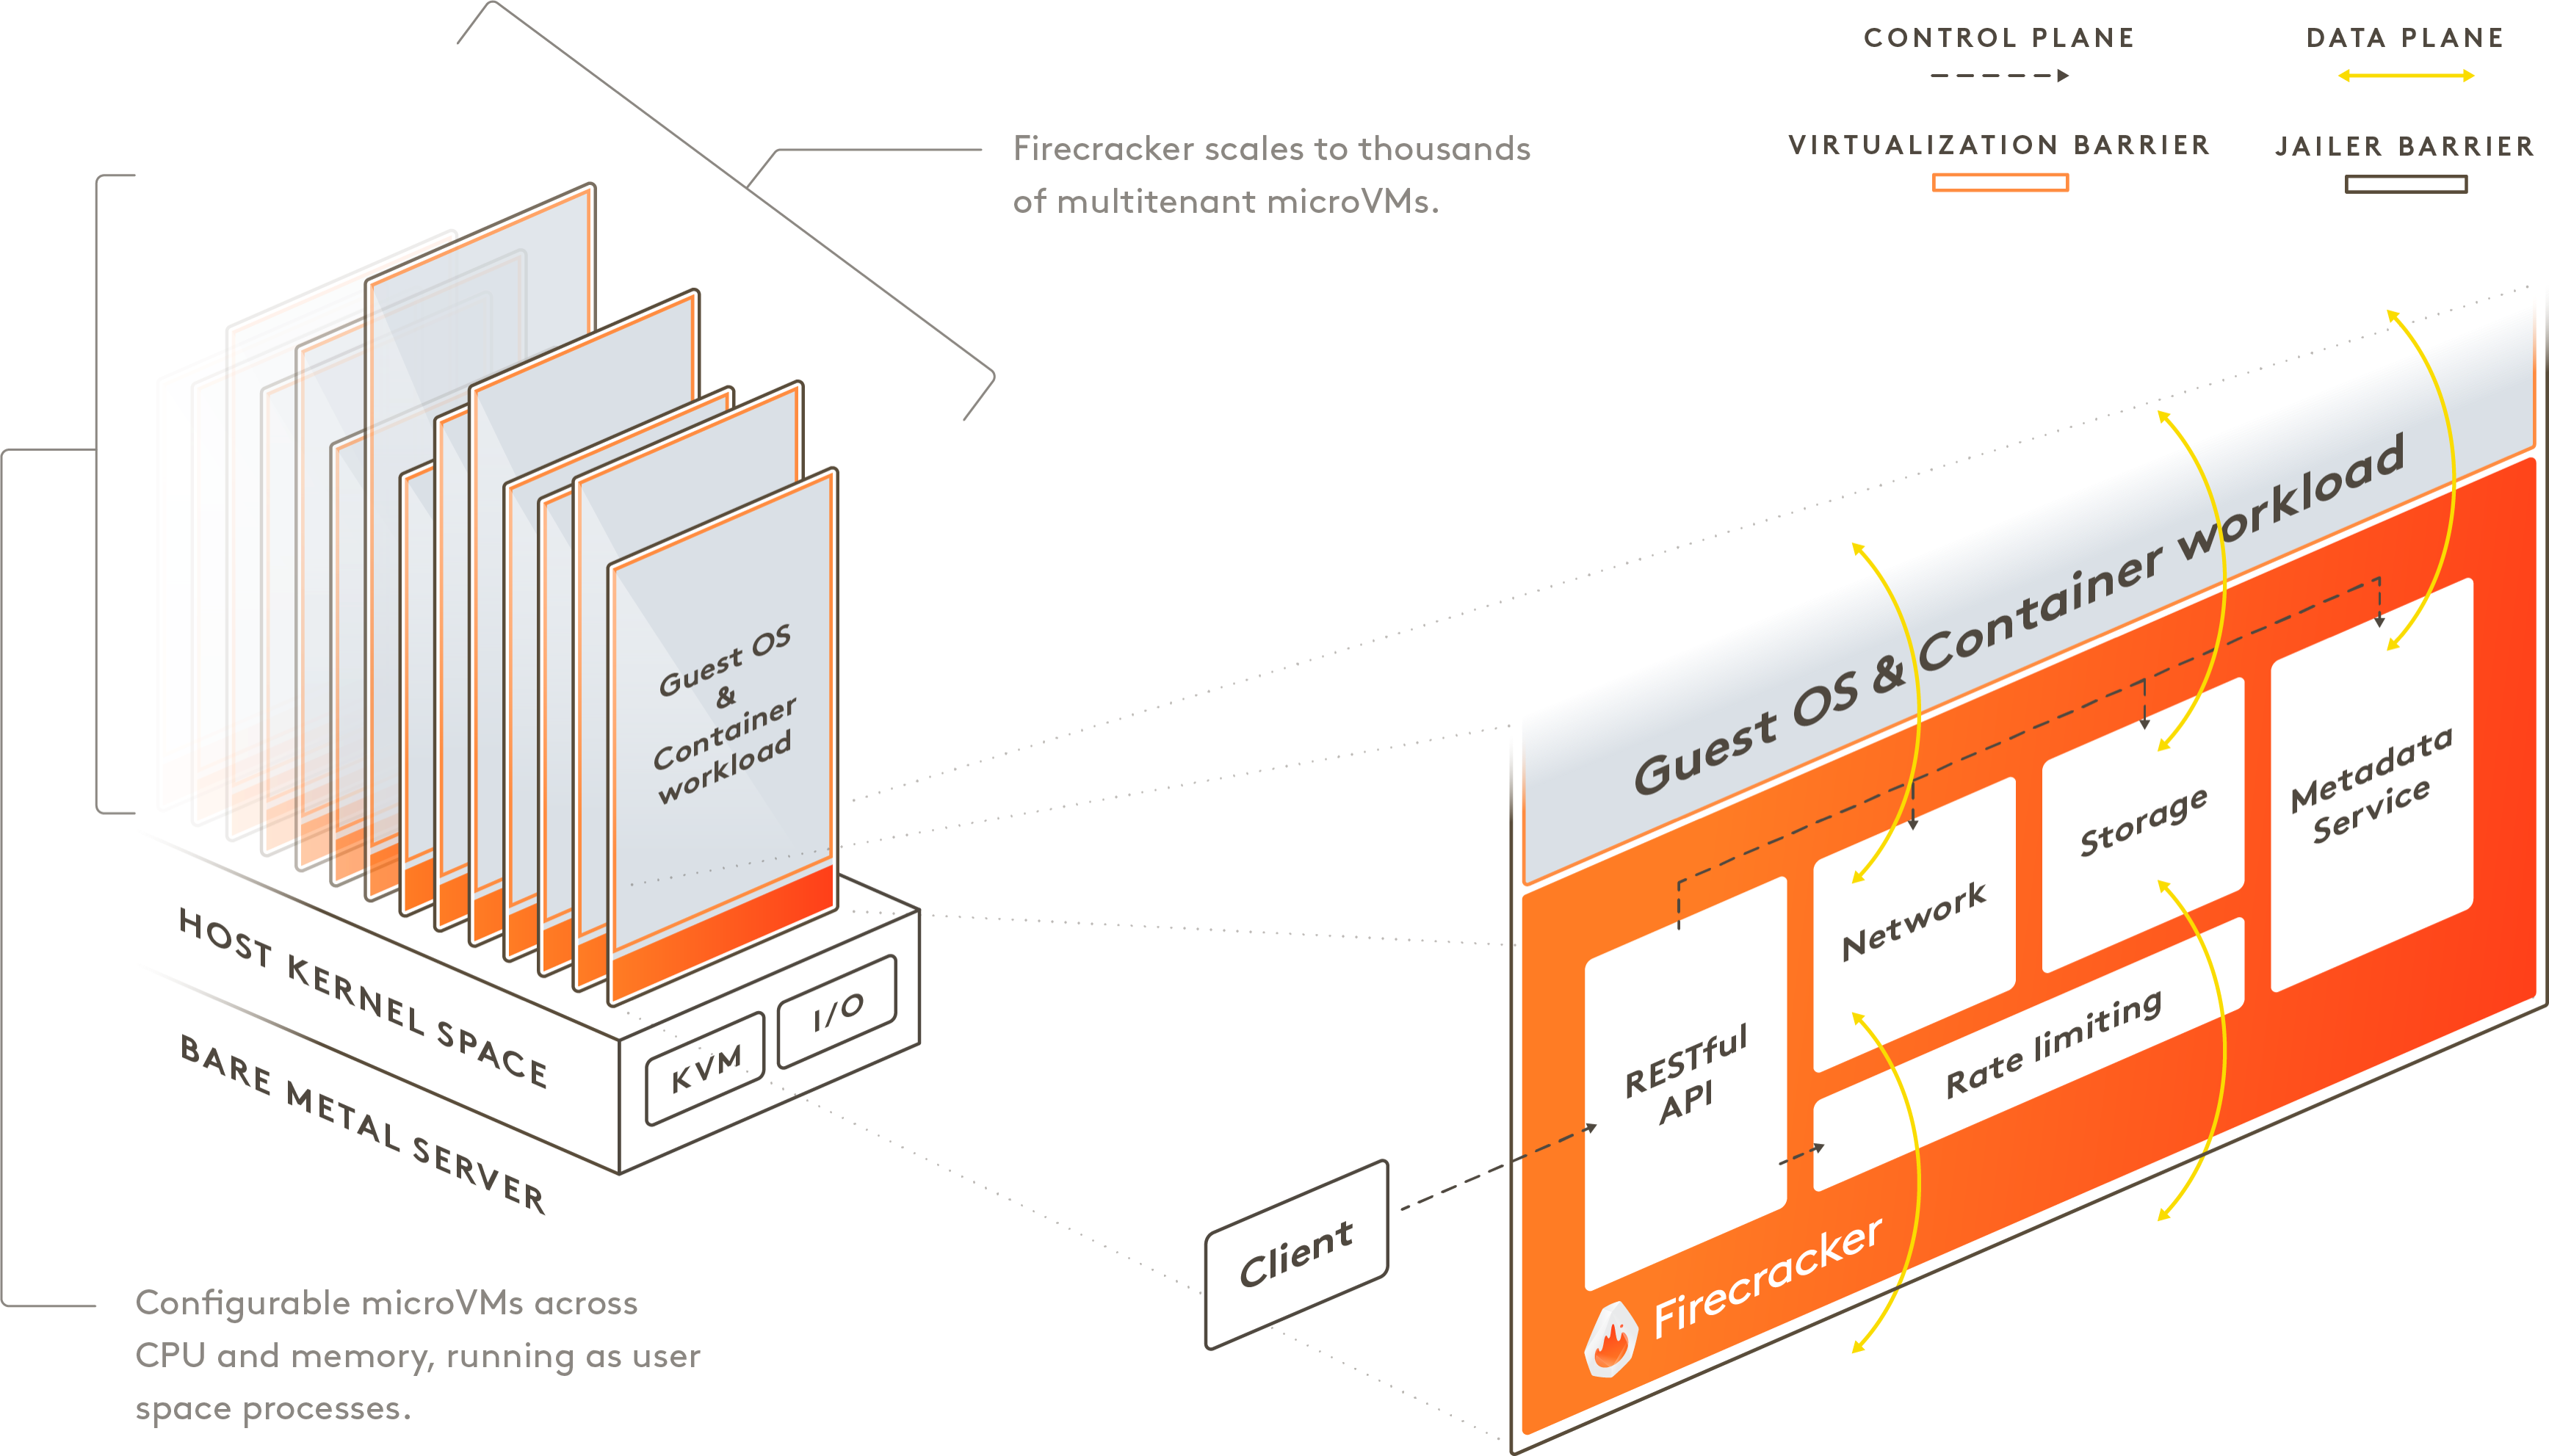
\includegraphics[width=0.8\linewidth]{figs/firecracker}
		\caption{}
		\label{figs:fire}
	\end{subfigure}
	\caption{}
	\label{figs:Firecracker}
\end{figure}
注意到图\ref{figs:internal}中特意标出了两个边界。内围的浅红色边界为Virtualization Barrier,利用虚拟化技术提供Customer Zone一个安全隔离的环境。外围的深红色的边界为Jailer Barrier,作为第二道防线,负责利用Linux提供的seccomp、cgroup、chroot、net/pid/user namespaces来创造沙盒环境;接着咋其创造的沙盒环境中启动Firecracker VMM;最后,Firecracker VMM利用KVM创建含有设备模型等(见上文第2点)的极度精简微虚机(Firecracker Zone)。

Firecracker的开发者与开源社区有着积极的互动。而从这篇报告完成的时间2020年5月底,在Firecracker主页上,我们已经惊喜的发现:Firecracker已经和Kata Containers、Weave FireKube集成在了一起,通过firecracker-containerd实现与容器的对接。图\ref{figs:fire}展示了Firecracker VMM的整体架构。集成了上文所述的图\ref{figs:host}\ref{figs:internal}中的要素,也集成了容器的工作负载。这三幅子图中,虽然一些表述不同,但是含义是一致的,如\ref{figs:host}中的Guest(绿色方框)、\ref{figs:internal}中的Customer Zone(红色方框)、\ref{figs:fire}中的Guest OS \& Container workload(灰色方框)表示的是同一个意思。而且如果把\ref{figs:internal}由Jailer Barrier围住的方框倒过来,和图\ref{figs:fire}的右边结构(包括内外围的两个Barriers)就几乎是一模一样的。另外,图\ref{figs:fire}中左边的结构画的非常的形象——和店面中出租的共享手机充电插槽设备神似。Firecracker的底座Host Kernel Space上面上可以插上千个多租户的微虚机,而且各个微机的规模大小是可以层次不齐的,代表了工作负载量。

\newpage
\section{Microsoft Serverless Computing(汪钇丞)}
\subsection{Azure}
Azure是微软的云平台,如图\ref{figs:Overview}所示,它根据不同层次的用户需求,提供了丰富和灵活的端到端服务\cite{overview}。Azure认为无服务器计算最主要的特点也是优点在于:开发者无需管理基础结构,而更多地专注于业务逻辑,能够在更短时间内交付更多功能;云服务提供商根据运行代码的工作负荷,自动预配、缩放和管理运行环境。Azure提供了符合上述特性的三种级别的抽象:Platform-as-a-Service(PaaS)、Functions-as-a-Service(FaaS)、Kubernetes-as-a-Service(KaaS),被认为是Azure的无服务器计算的三个主要组成部分。
\begin{figure}[!htbp]
	\centering
	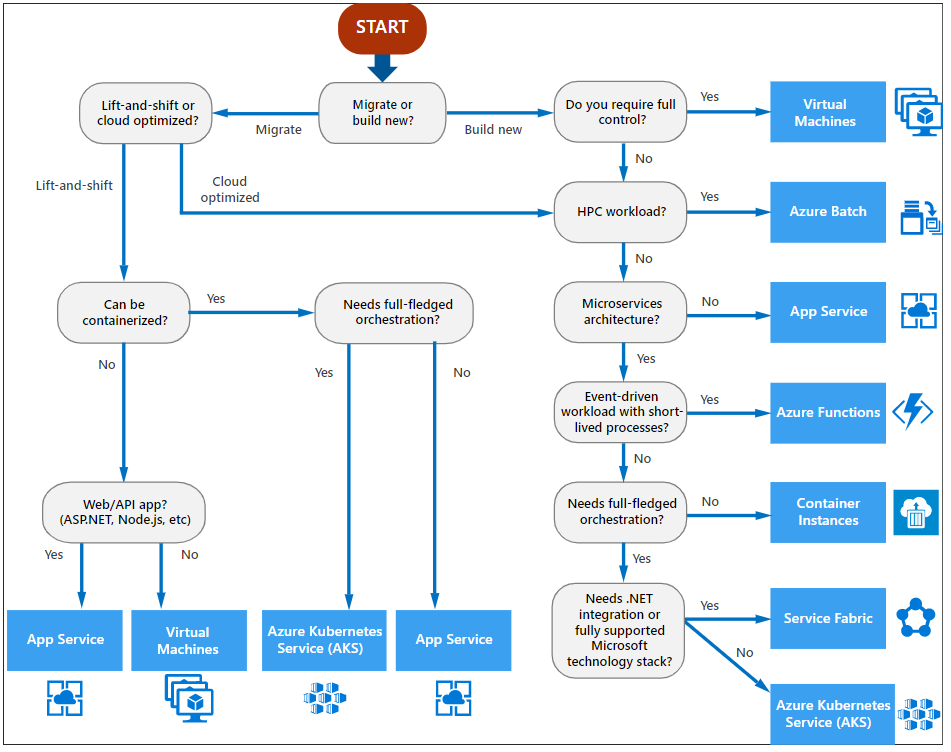
\includegraphics[width=0.7\linewidth]{figs/AzureChoice.PNG}
	\caption{Azure根据需求提供的功能选择(\cite{overview}图1)}
	\label{figs:Overview}
\end{figure}

\subsection{Azure App Service}
Azure App Service是Azure提供的平台即服务(PaaS),相比较与基础架构即服务(Infrastructure-as-a-Service)需要用户自行修补和备份服务器,安装软件包,更新操作系统和监视应用程序,Azure App Service中由运营商来做上述的工作来维护虚拟机环境,用户只需要选择一个基于HTTP请求的平台目标,例如Web应用,REST API,或者移动后端等。

随着应用对后台处理的需求增加,微软引入了Azure WebJobs作为Azure App Service的拓展。WebJobs 作为一个工作流程步骤,它含有基于时间的触发器,以及基于Azure提供的存储系统,数据库,消息队列等工具的触发器,可以持续执行,通过触发执行,或者是手动触发执行特定的逻辑任务。Azure WebJobs本身已经具有了一些典型无服务计算运行时的特点,可以说是一个FaaS平台的雏形,但WebJobs SDK的编写相对来说还是较为繁琐,监视和日志系统也不够完善。

相比较于其他PaaS平台,Azure App Service的特点在于可以支持包括ASP.NET,JAVA,Ruby,Node.js,PHP,Python在内的多种编程语言;能够使用微软自家Visual Studio中的专用工具,简化了创建,部署和调试工作;可以使用Azure的DevOps进行持续集成和部署;能够使用Azure Active Directory进行身份验证确保安全性;可以从Azure市场上获取到大量应用程序的模板。最关键的一点是,Azure App Service 除了在基本付费计划当中需要用户手动伸展和收缩集群,在标准和高级付费计划当中,都提供了自动化集群和实例数量伸缩的功能选项,让用户无需再关注应用运行环境,这一特点使得Azure App Service具有了无无服务器计算的性质。


\subsection{Azure Functions}
Azure Functions是Azure提供的函数级别的抽象(Function as a Service),一个典型的事件驱动型无服务计算运行时。如图\ref{figs:architecture}所示,Azure Functions建立在Azure App Service和WebJobs SDK的基础之上,相当于一个轻量级的WebJobs SDK脚本模型。它利用触发器自动执行代码以响应事件或绑定,能够根据工作负载量自动灵活地缩放计算资源,无需基础结构管理。相对于WebJobs只能跟随Azure App Service运行在公有云之上,Azure Functions既可以运行在Azure公有云上,也可以通过Azure Stack运行在自有混合云平台中,常常在Azure App Service 中作为服务的一部分。

\begin{figure}[!htbp]
	\centering
	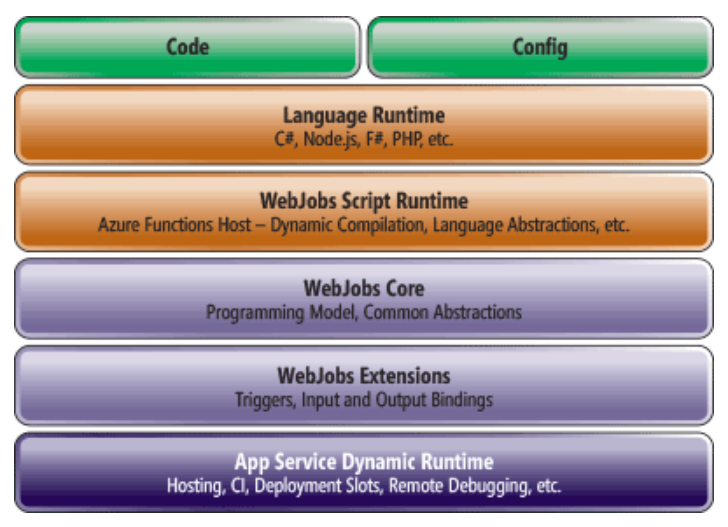
\includegraphics[width=0.5\linewidth]{figs/AzureArchitecture.PNG}
	\caption{Azure App Service体系结构(\cite{archi}图1)}
	\label{figs:architecture}
\end{figure}

\subsubsection{Azure Functions触发器}
触发器是启动函数的按钮,定义函数如何被调用,为请求提供标准的跨平台有效负载。每个函数有且只有一个触发器。Azure Functions可以响应的触发包括:
\begin{enumerate}
	\item HTTP:基于HTTP请求运行代码, Azure API Management将云服务的所有后端服务API网关中心化,可以集中接收HTTP请求。
	\item 计时器:基于时间调度在预定的时间执行代码,可以满足周期性的触发,用于监视系统等。
	\item 数据库:连接Azure的全球分布式的多模型NoSql数据库Azure Cosmos DB。基于该数据库文档的增删改情况运行代码。
	\item 存储系统:连接了Azure存储HTML,CSS等静态Web内容的Azure Blob存储,消息队列Azure Queue,表格Azure Table等。基于这些存储的增删改情况运行代码
	\item Event Grid:事件网格是Azure完全托管的事件路由服务,使用发布/订阅模型,收集和传递多个主题源发布的事件。基于事件网格订阅的一系列事件来进行反馈
	\item Event Hub:Azure面向loT领域收集设备和传感器数据的中心,基于物联网设备的大量数据输入,运行代码进行反馈
	\item 服务总线:连接其他Azure或者自有的服务以及设备,对总线中的消息队列等作出反馈
\end{enumerate}
\subsubsection{Azure Functions绑定}
Azure通过Azure Logic Apps以低编码/无编码的方式,集成连接了各类软件,应用以及Software as a Service等服务,使得Azure Functions可以直观的创建无服务器工作流,将云中的数据连接并集成,提供给Azure Functions当中作为工作负载。如图\ref{figs:bind}所示,Azure Functions通过显式声明的方式进行绑定,将另一个微软的资源连接到函数当中。绑定可以是输入绑定、输出绑定或者都绑定。绑定对于Azure Function是可选的,一个函数可能有一个或多个输入和输出绑定。绑定的输入可以来自Azure的存储系统,数据库,微软的表格,云盘等等。输出除前述的资源之外还可以是通向事件网格,物联网中心,微软的邮件系统等。
\begin{figure}[!htbp]
	\centering
	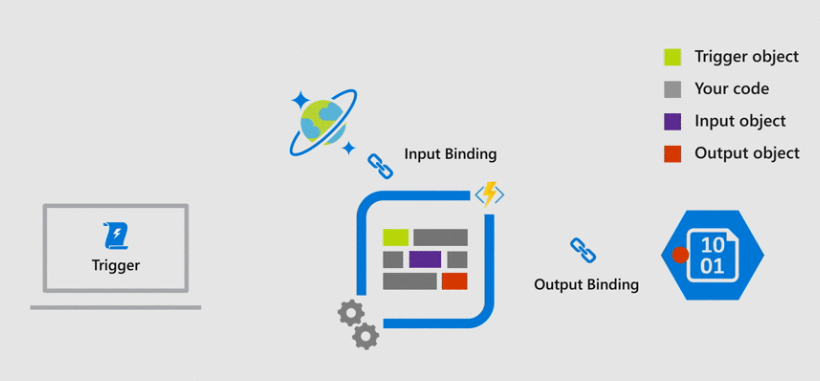
\includegraphics[width=0.6\linewidth]{figs/AzureBindings.png}
	\caption{Azure Functions Binding示意图。\cite{binding}图2)}
	\label{figs:bind}
\end{figure}
\subsubsection{Azure Functions安全和监控}
Azure Application Insights是一个无服务器诊断平台,作为Azure Monitor功能的一部分,内置在Azure Functions当中作为一种服务提供。它不需要额外配置服务器或设置库,自动与应用集成,负责监控和分析代码性能,可以收集日志,性能数据和错误信息,自动检测性能异常,诊断问题并了解函数的使用情况,给出解决意见。通过应用程序图和分布式跟踪,在应用程序的所有组件中发现任务热点,任务瓶颈和故障,并通过非常人性化的UI展示。除了内置的遥控跟踪可供控制,也可以自定义统计信息,设置日志级别,生成定制的遥控跟踪项目。

而作为Azure App Service的一部分,Azure Functions也是通过Azure Active Directory,或者Microsoft帐户和外部提供商的内置身份验证授予应用程序访问权限,并通过Azure Key Vault全面控制访问策略和审核历史记录。除此之外的Azure Functions的高级付费计划中提供了独立隔离的虚拟网络Azure VNet,可以限制进入的流量。Azure Security Center则负责预防、检测和响应威胁,增强对Azure 资源安全的可视化和可控性。
\subsubsection{Azure Functions的付费计划}
针对不同的应用场景和需求,Azure Functions提供了三种不同的付费计划,不同的计划也决定了函数的伸缩方式,每个函数实例的可用资源,以及对Azure VNet的可支持性。
\begin{itemize}
	\item Consumption计划:最典型的无服务器计算付费计划,仅当函数运行时,基于执行的实例数量、执行时间和执行所用内存大小为计算资源付费。Azure会根据传入事件的数量动态添加和删除Azure Functions主机的实例,自动扩展
	\item Premium计划:适用于函数一直连续执行的情况,计划会保持至少一个永久热的实例在运行,以避免冷启动,意味着费用计算会有最低成本。除此以外用户可以选择连接Azure VNet,选择实例所用的CPU核数量,并拥有无限执行时间(至少60分钟)而不会超时
	\item Dedicated计划:实际上就是分享Azure App Service的资源,如果Azure App Service的付费计划中的虚拟机没有被充分利用,则用来创建Azure Functions实例。这也意味着虚拟机会一直在线。
\end{itemize}
Consumption计划和Premium计划根据创建的函数实例数来伸缩所需的CPU和内存资源,伸缩的单位就是一个函数实例,Azure Functions使用一个伸缩控制器监测触发事件,并启发式地控制伸缩大小,伸缩范围从0个实例到200个实例,每个实例可以处理很多个请求。对HTTP触发器每秒最多增加一个实例,而对非HTTP触发器最快每30秒增加一个实例。而Dedicated 计划则默认的是手动伸缩,也可以在对应App Service 计划中选择自动伸缩。另外Azure Functions依赖Azure存储来管理触发器和记录函数执行等,所以用户必须要有一个支持Azure Blob, Queue, Files, and Table storage的Azure存储账户。

\subsubsection{Azure Functions的性能}
Azure Functions作为微软的商用无服务器计算运行时,它的具体实现集成了众多Azure服务,并是不开源的。因而现有的相关论文的研究方法包括有:利用Azure的基本服务和工具,以及其他的开源项目有,重新搭建出一个FaaS的原型\cite{mcgrath2017serverless};或是直接测试Azure Functions 的进行测试,尝试逆向构建并了解其性能特点\cite{wang2018peeking}。

\cite{wang2018peeking}{\textit{Wang等人发表在USENIX ATC’18的文章}}对Azure Functions的性能和可用性进行了更深入的评测。他们首先根据官方文档找到了一个环境变量,由它能够确定Azure用于执行函数的虚拟机ID,论文使用两个不同的账号,分别触发500次函数,然而发现有30\%的函数实例是与另一用户的函数实例共存在同一个虚拟机上的。由于同一虚拟机共享相同的资源,这种共存情况为数据安全带来了一定隐患,会导致应用程序容易受到各种各样的边通道攻击。

而在更大规模的50000次的函数调用测试当中,论文总共统计到4104个不同的虚拟机,三种不同的CPU,以及有单核,双核,四核三种配置。根据Azure官方付费计划中的叙述,一个计划内可以最多拓展到200 个实例,但实际在测试当中,不论作者如何调整,整体的实例数也没有超过10个,且都不在同一个虚拟机上,说明Azure不会在同一虚拟机上申请相同函数的实例,造成绝大多数的申请都是由个别实例完成的。

当\cite{wang2018peeking}采用同一账户调用100个不同的函数,使总的函数实例数达到1000个时,论文查看所有实例的虚拟机分布,发现只有最多8个实例能够独享一台虚拟机,绝大部分的实例都会和其他实例共享虚拟机,并且大部分共享的虚拟机都是在单核环境,而不是在其他双核和四核虚拟机上。这表明Azure提供了更多的低性能单核虚拟机,而有实例共享虚拟机的情况都发生在单核虚拟机上,会带来更大的竞争。论文随后采用两个账户,一个触发少量函数实例扮演“受害者”,一个同时产生大量函数实例作为“侵略者”,作者发现有部分“受害者”的实例会和“侵略者”的实例共享虚拟机的情况,由此产生性能损失。
\begin{figure}[!htbp]
	\centering
	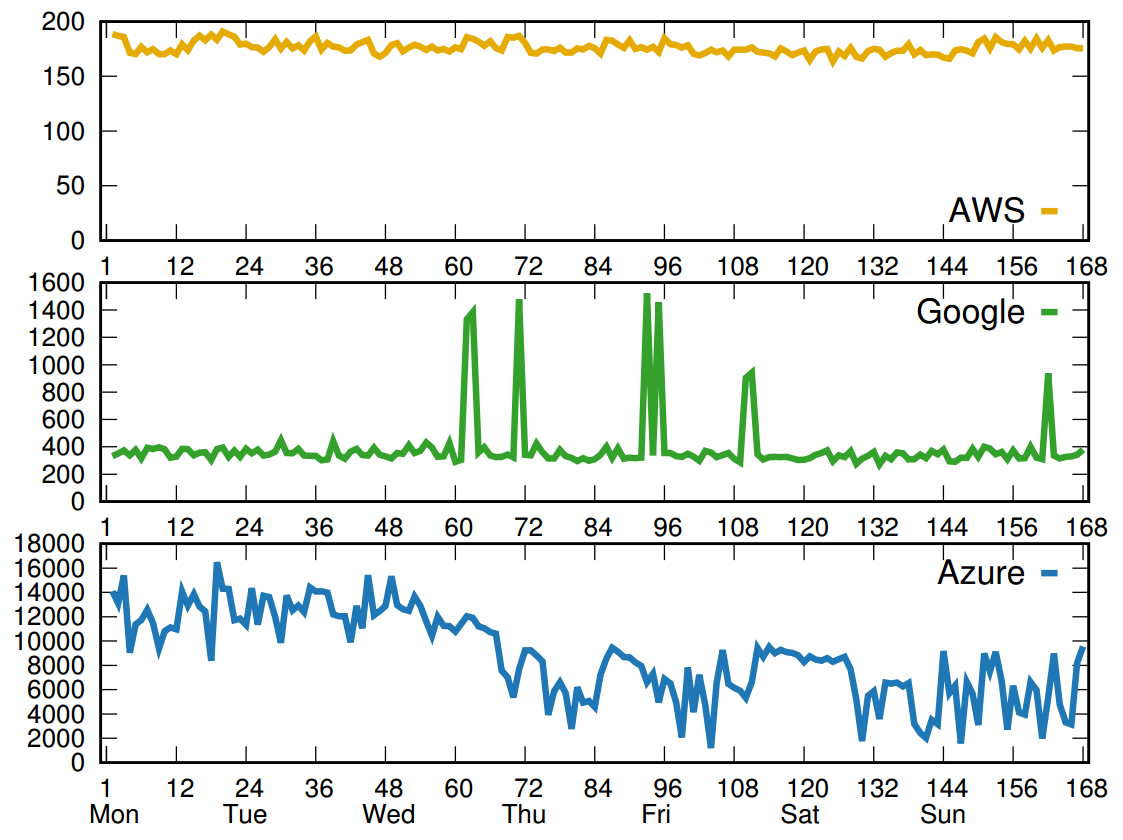
\includegraphics[scale=0.5]{figs/ColdStart.PNG}
	\caption{主流FaaS平台的冷启动延迟对比(\cite{wang2018peeking}图8)}
	\label{figs:cold}
\end{figure}

冷启动指的是未经使用或长时间没有使用的应用程序,由于需要重新分配和加载而启动时间较长的现象。在冷启动现象的测试中,\cite{wang2018peeking}对1000种不同的函数,连续调用两次,分别作为冷启动和热启动的比较。结果显示,和同类型的AWS和Google产品相比较,尽管Azure每个函数实例分配了更多内存,但冷启动延迟的中位数要远远高出,并且相对来说延迟时间更不稳定,如图\ref{figs:cold} 所示。而作者统计了一个函数实例在运行结束后到被回收掉的时间,发现Azure的回收间隔时间则相对较短,这意味着Azure的资源利用效率更高,但新的相同函数请求找到一个热实例的可能性更小。不过在存活实例的最长生命时间实验中,Azure函数实例在保持存活的情况下,在虚拟机中的最长存在时间要明显高于另外两个产品。

在单独的虚拟机性能方面,Azure的函数实例的CPU占用率,I/O,网络吞吐量方面和其他两款产品差异不大,但由于Azure提供的虚拟机并不一致,相对来说四核的虚拟机性能更佳,CPU资源占用率更高,而单个实例的I/O和网络吞吐会随着实例共享而下降。因而Azure Functions的性能相对来说并不稳定。

\cite{wang2018peeking}的测试都是针对Consumption计划,在论文撰写时Premium计划还没有推出。而Premium计划的提供已经解决了避免冷启动的问题,方法是至少保持一个热实例,也通过隔离的虚拟网络Azure VNet 和可配置的CPU核数量,保证了没有不同用户共享虚拟机的情况出现,避免了实例之间的竞争,虚拟机的性能也可以得到保证。论文在最后也说明最新的测试证明了Azure Functions更新的有效性。而Dedicated 计划则可以完全避免冷启动,因为虚拟机是由用户控制的,但这种情况之下就不再是无服务器的了。

\subsection{Azure Kubernetes Service}
Kubernetes是一个用于自动部署,扩展和管理容器化应用程序的开源系统。它提供API来控制容器的运行方式和位置.自动进行服务发现、负载均衡、存储编排、部署和回滚、自我修复、跟踪资源分配和基于计算利用率进行扩展。而Azure Kubernetes Service(AKS)是Azure提供的Kubernetes即服务(KaaS),用于托管Kubernetes环境,使在Azure中部署和管理容器化的应用程序变得容易。由于不需要关注具体的容器管理,能够自主伸缩,因而AKS也被视为微软无服务器计算的一部分。
\begin{figure}[!htbp]
	\begin{subfigure}[b]{0.38\linewidth}
		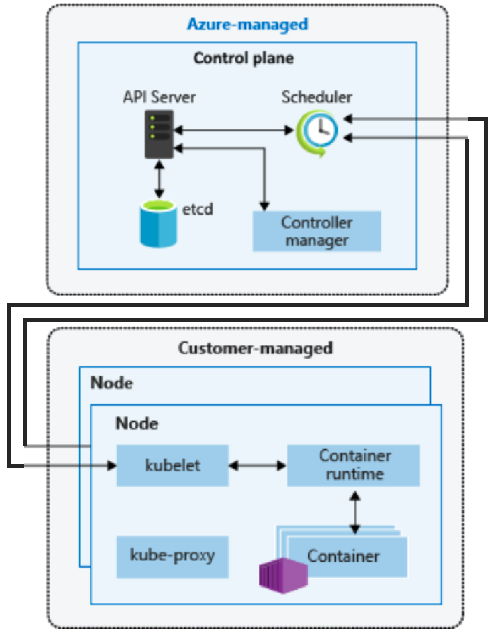
\includegraphics[width=\linewidth]{figs/Kubernetes}
		\caption{}
		\label{figs:Structure}
	\end{subfigure}
	\begin{subfigure}[b]{0.62\linewidth}
		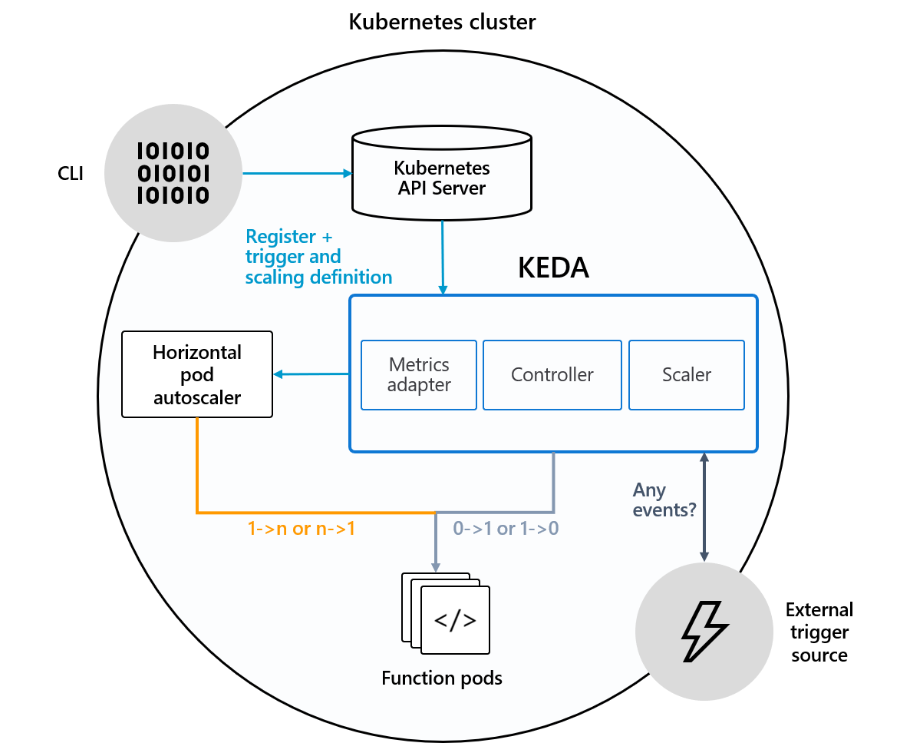
\includegraphics[width=\linewidth]{figs/KEDA}
		\caption{}
		\label{figs:KEDA}
	\end{subfigure}
	\caption{(a) Kubernetes的结构图。(b) KEDA的结构图。(\cite{Kubernetes})}
\end{figure}

\subsubsection{Kubernetes结构}
Kubernetes的结构如图\ref{figs:Structure}所示,其结构的主要组成包括:
\begin{itemize}
	\item 控制平台:也就是主节点,由许多小型专门的控制循环和服务组成。其中API Server是底层Kubernetes API的公开方式。为管理工具(如kubectl或Kubernetes dashboard)提供交互;Cluster store是为维护Kubernetes集群状态和配置的一个高度可用的KV结构etcd存储;Scheduler在创建或扩展应用程序时,根据工作负载确定哪些节点可以运行并启动它们;Controller-Manager监督许多更小的控制器,提供自愈能力、扩容、应用生命周期管理、服务发现、路由、服务绑定和提供。
	\item Nodes节点:Kubernetes集群的工作节点,负责查看API服务器以获得新的工作分配,执行新的工作分配,并向控制平面报告。其中kubelet负责节点注册过程,监视API Server来得到分配的工作,并将容器的运行状态汇报给API Server;Container Runtime负责镜像管理以及Pod和容器的真正运行;kube-proxy负责为Service提供cluster内部的服务发现和负载均衡,通过iptables规则引导访问到服务IP,并将其重定向至正确的后端应用
	\item 容器都运行在Pod内部,而一个Pod运行一个应用的实例。Pod通常与容器进行1:1的映射,高级场景中一个Pod也可能包含多个容器。这些多容器容器被安排在同一个节点上,允许容器共享相关资源,相同的Pod将共享相同的IP 地址。创建一个Pod 时,可以定义资源请求来申请一定数量的CPU或内存资源。Scheduler尝试将pod调度到具有可用资源的节点上运行,以满足请求。Pod是伸缩的最小单元。如果要伸缩应用程序,可以添加或删除Pod,不能通过向现有的Pod添加更多容器。由于Pod是不可靠的,Pod的伸缩也可能很耗费IP地址,Service为Pods集合提供可靠的网络
\end{itemize}

\subsubsection{AKS特征}
AKS的控制平面由Azure来负责控制,并保证是单租户使用的,而只需为运行应用程序的Node付费,而集群的Node数量是至少3 个。受托管的控制平面意味着用户不需要配置高度可用的etcd存储等组件,但是它也意味着不能直接访问主节点。AKS建立在开源的Azure Kubernetes 服务引擎(AKS-Engine)之上,使用Moby作为容器运行时,在包含多个节点池的AKS集群中,需要告诉Kubernetes 调度器将哪个节点池用于给定的资源。相比于传统Kubernetes,AKS可以将Azure存储等工具连接到节点和Pods,可以使用GPU,可以利用之前提到的Azure Active Directory,监视和诊断之类的功能。另外AKS提供了虚拟节点,无需等待Kubernetes集群的自动缩放器部署VM计算节点,即可快速运行虚拟节点上热启动的Pod,而只为它们的执行时间付费。

\subsubsection{基于Kubernetes的事件驱动自动缩放}
基于Kubernetes的事件驱动自动缩放器(即KEDA),可以指定应用程序以事件驱动方式扩展,根据需要处理的事件数确定如何扩展Kubernetes中的任何容器。作为一个单一用途的轻量级组件,它可以添加到包括AKS在内的任何Kubernetes集群中,与标准Kubernetes组件一起使用,而不会覆盖或重复原有功能。KEDA自动伸缩,事件驱动的特点,与Azure Functions的性质吻合,因而安装KEDA的AKS也是Azure Functions的一种可用托管方式,通过Kubernetes中提供事件驱动的缩放。Kubernetes自身通过Horizontal Pod Autoscaler定期查询内存和CPU资源的利用率等评价指标来决定伸缩的程度,最终计算得到应该创建的实例数。而Kubernetes从1.6版本开始支持添加自定义的指标,KEDA将触发对象的状态,例如Azure消息队列的长度,定义为评价指标,添加到指标服务器中提供给Horizontal Pod Autoscaler,做到启发式的Pod实例伸缩。如图\ref{figs:KEDA} 所示,KEDA的功能实现主要依靠三个组件:
\begin{enumerate}
	\item Scaler:通过自定义资源ScaledObject的manifest定义,和外部触发对象的工具连接,负责获取定义的指标并提供给指标服务器,KEDA支持同时插入多个Scaler
	\item Controller:负责初始部署,完成实例从0到1和从1到0,通过KEDA-operator容器驱动,在自定义的资源ScaledObject出现之后,创建一个Horizontal Pod Autoscaler。
	\item Metrics Adapter:即指标服务器,通过将Scaler提供的指标数据进行一定的处理,提供给相应的Horizontal Pod Autoscaler,由后者来根据指标对Pod实例数量进行伸缩。
\end{enumerate}
KEDA目前可支持的触发对象包括Azure存储队列,Azure服务总线队列,Azure时间网格,以及Apache Kafka等开源项目。但相比较于Azure Functions的原生计划来说还并不完整,如不支持计时器触发,HTTP请求等,或者是需要其他繁琐的插件来支持。

\newpage
\section{(胡登杭)}
\subsection{Durable Azure Functions}
Durable Functions 是 Azure Functions 的一个扩展,可用于在无服务器计算环境中编写有状态函数。  
有几种典型的应用模式:
\subsubsection{模式 1:函数链}
在函数链接模式中,将按特定顺序执行一系列函数。 在此模式中,一个函数的输出将应用到另一函数的输入。
\begin{figure}[!htbp]
	\centering
	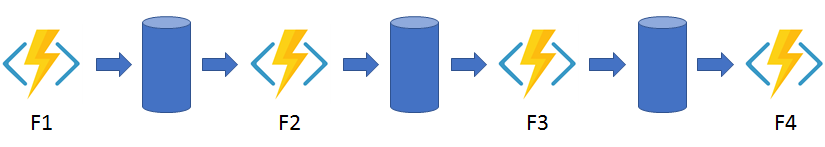
\includegraphics[width=0.8\linewidth]{figs/model1}
	\caption{函数链(\cite{Durable})}
\end{figure}

\subsubsection{模式 2:扇出/扇入}
在扇出/扇入模式中,将会并行执行多个函数,然后等待所有函数完成。 通常会对这些函数返回的结果执行一些聚合操作。
\begin{figure}[!htbp]
	\begin{subfigure}[b]{0.62\linewidth}
		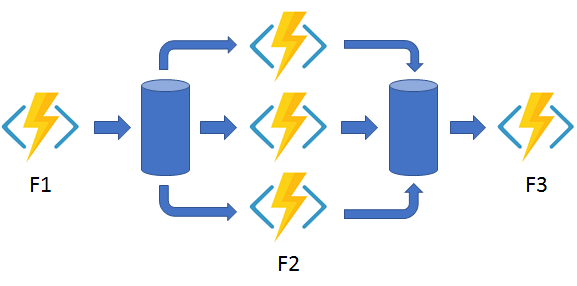
\includegraphics[width=\linewidth]{figs/model2}
		\caption{}
	\end{subfigure}
	\begin{subfigure}[b]{0.38\linewidth}
		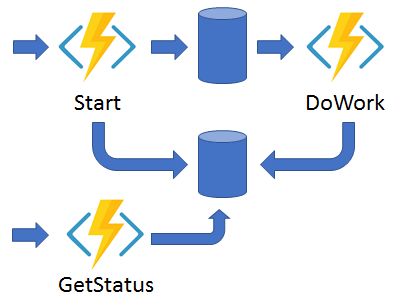
\includegraphics[width=\linewidth]{figs/model3}
		\caption{}
	\end{subfigure}
	\caption{(a) 扇出/扇入。(b) 异步 HTTP API。(\cite{Durable})}
\end{figure}

\subsubsection{模式 3:异步 HTTP API}
异步 HTTP API 模式解决了使用外部客户端协调长时间运行的操作的状态时出现的问题。 实现此模式的一种常用方式是让 HTTP 终结点触发长时间运行的操作。 然后,将客户端重定向到某个状态终结点,客户端可轮询该终结点,以了解操作是何时完成的。

\subsubsection{模式 4:监视}
监视模式是指工作流中的灵活重复进程。 例如,轮询到满足特定的条件为止。 可以使用常规计时器触发器解决简单方案(例如定期清理作业),但该方案的间隔是静态的,并且管理实例生存期会变得复杂。 可以使用 Durable Functions 创建灵活的重复间隔、管理任务生存期,以及从单个业务流程创建多个监视进程。
监视模式的一个例子是反转前面所述的异步 HTTP API 方案。 监视模式不会公开终结点供外部客户端监视长时间运行的操作,而是让长时间运行的监视器使用外部终结点,然后等待某个状态发生更改。

\subsubsection{模式 5:人机交互}
许多自动化过程涉及到某种人机交互。 自动化过程中涉及的人机交互非常棘手,因为人的可用性和响应能力不如云服务那样高。 自动化过程允许使用超时和补偿逻辑来实现这种交互。
审批过程就是涉及到人机交互的业务过程的一个例子。 例如,某份超出特定金额的开支报表需要经理的审批。 如果经理未在 72 小时内审批该开支报表(经理可能正在度假),则会启动上报过程,让其他某人(可能是经理的经理)审批。
\begin{figure}[!htbp]
	\begin{subfigure}[b]{0.28\linewidth}
		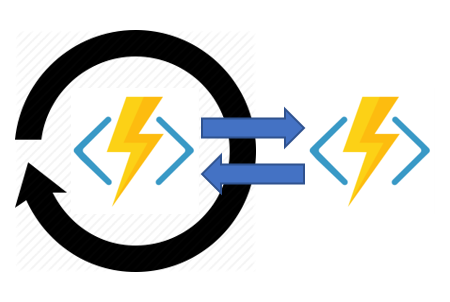
\includegraphics[width=\linewidth]{figs/model4}
		\caption{}
	\end{subfigure}
	\begin{subfigure}[b]{0.36\linewidth}
		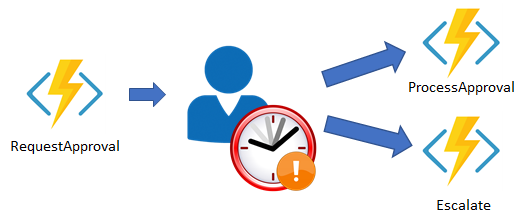
\includegraphics[width=\linewidth]{figs/model5}
		\caption{}
	\end{subfigure}
	\begin{subfigure}[b]{0.36\linewidth}
		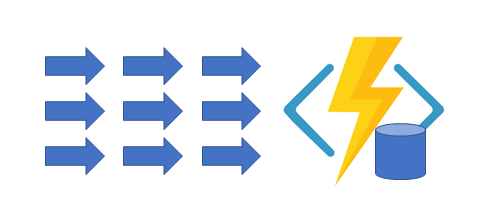
\includegraphics[width=\linewidth]{figs/model6}
		\caption{}
	\end{subfigure}
	\caption{(a) 监视。(b) 人机交互。(c) 聚合器。(\cite{Durable})}
\end{figure}

\subsubsection{模式 6:聚合器(有状态实体)}
第六种模式涉及到将一段时间的事件数据聚合到单个可寻址的实体。 在此模式中,要聚合的数据可来自多个源、可分批传送,也可以分散在较长的时间段。 聚合器可能需要在事件数据抵达时对其执行操作,而外部客户端可能需要查询聚合数据。

\subsection{Azure Data Lake Store}
\subsubsection{Azure Data Lake Analytic}
Azure Data Lake Store(ADLS) 是微软针对Azure Data Lake Analytic(ADLA)研发的一套存储系统。所以在了解ADLS之前,我们先了解一下ADLA.\\
Data Lake, 中文翻译为数据湖。五湖四海,海纳百川,湖泊象征着广博,象征着纷繁复杂。所以顾名思义数据湖代表一类没有经过处理的、杂乱的原始数据。为了提取出数据中的有效信息,所以需要对数据湖进行"analytic",这就是Data Lake Analytic的含义。然而由于数据湖中的数据是原始的、未经过处理的,所以数据量会非常大,现代数据湖的数据量已经到了EB量级。为了能够分布式地存储和分析这么大量级的数据,微软研发了分布式存储系统ADLS。
\subsubsection{设计目标}
ADLS主要是为ADLA服务的,主要的设计目标跟数据湖分析的目标相似,有三点:1)处理高并发的读操作和写操作;2)低延时地处理高带宽的数据;3)存储大量数据(EB量级)。
\subsubsection{设计特色}
ADLS和HDFS一样是分布式存储系统,是Cosmos存储系统的一个延伸,它综合了HDFS和Cosmos存储系统优点。主要有两个特色:支持多种存储方式和特殊的文件存储方式。
\begin{figure}[!htbp]
	\begin{subfigure}[b]{0.5\linewidth}
		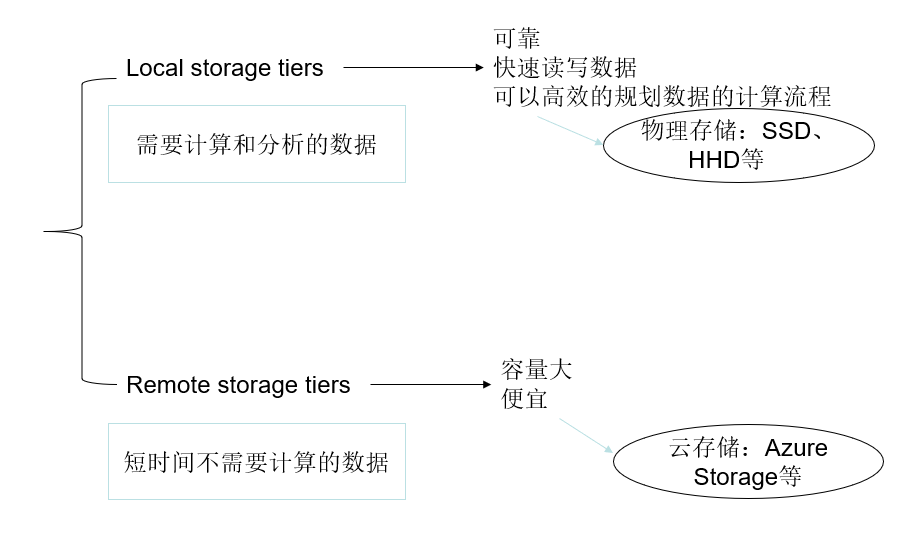
\includegraphics[width=\linewidth]{figs/data_store.png}
		\caption{}
		\label{fig:data_store}
	\end{subfigure}
	\begin{subfigure}[b]{0.5\linewidth}
		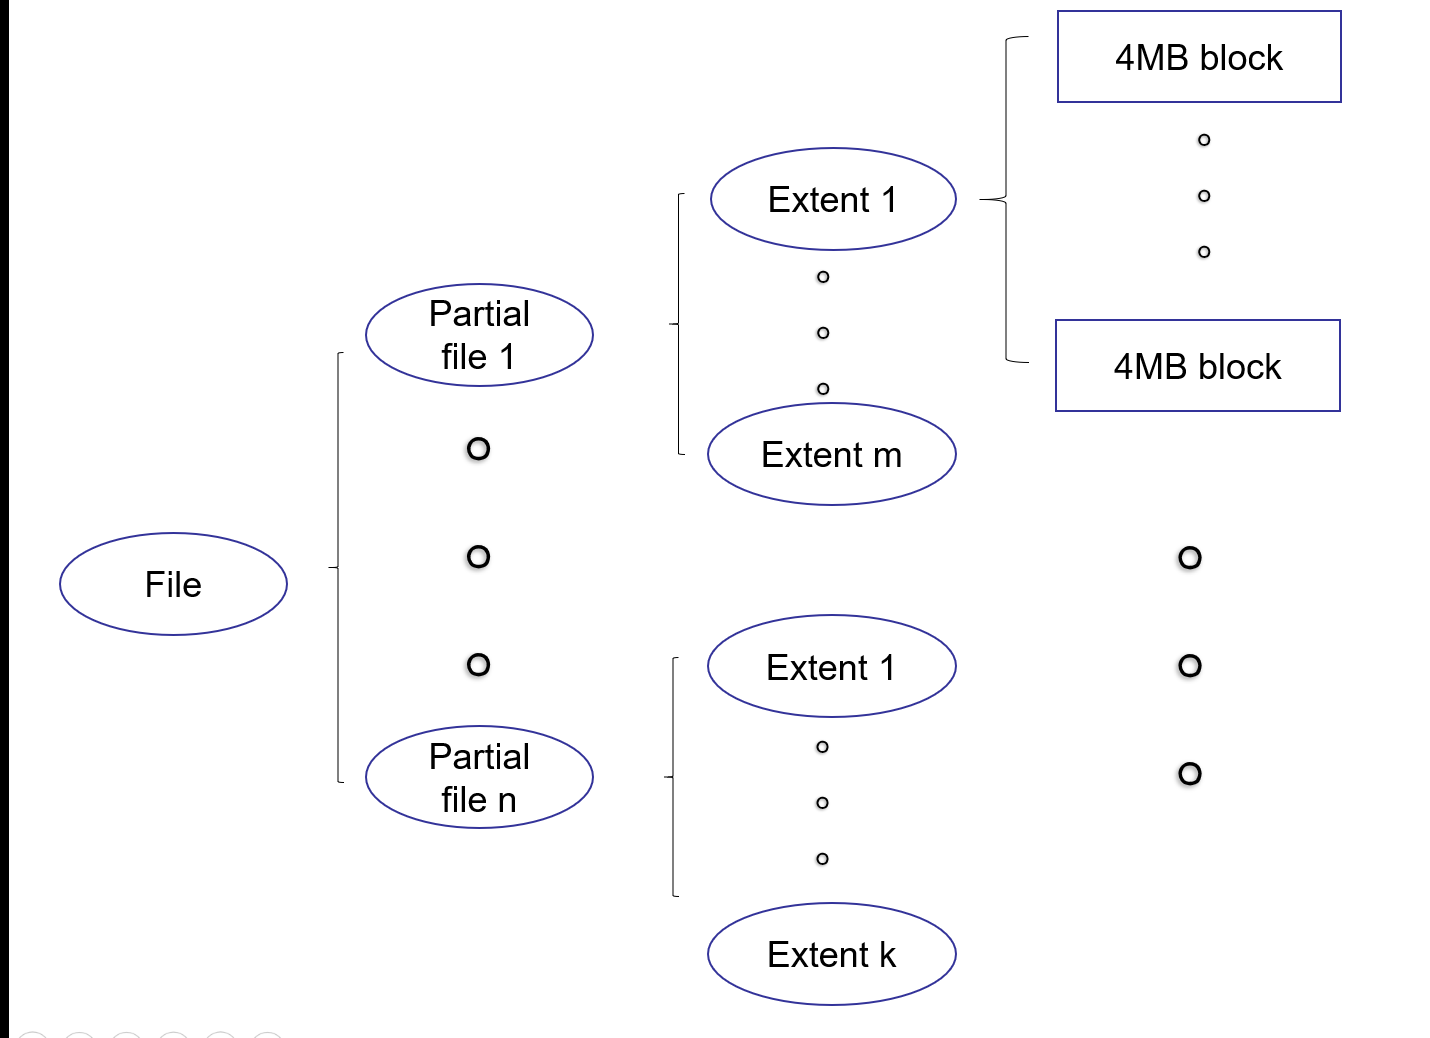
\includegraphics[width=0.8\linewidth]{figs/file_store.png}
		\caption{}
	\end{subfigure}
	\caption{}
\end{figure}
\begin{enumerate}
	\item \textbf{支持多种存储方式-物理存储和云存储}\ \ ADLS把存储系统抽象为Storage tiers, 每个tiers对应着一个特有的存储提供商。存储提供商可以是本地的物理存储如SSD,也可以是云存储如Azure Storage。如\ref{fig:data_store}所示,Storage tiers分为两种类型:Local storage tiers和 Remote storage tiers。
	\begin{itemize}
		\item Local storage tiers:本地存储层中的数据直接存储在ADLS内部节点中,如本地计算机的SSD中。这些数据可以被ADLS快速的访问,在做计算任务时也容易规划。所以一般把短时间内需要频繁计算和分析的数据放在本地存储层。
		\item Remote storage tiers:然而本地存储层的容量总是有限的,为了处理EB量级的数据,还需要借助其他云存储服务器的空间,称为远端存储层。远端存储层数据的访问较慢,数据通信较慢导致计算速度也慢,唯一的优点就是空间大。一般用来存储短时间不需要分析的数据。
	\end{itemize}
	\item \textbf{把每个文件分段存储}\ \ ADLS把每个文件细分为了partial file, 对每个partial file又细分为了extents,每个extents由多个4KB的数据块组成;目的是便于维护分布式读写操作的正确性。每个file、partial file和extent都有sealed和unsealed两个状态,定义如下:
	\begin{itemize}
		\item Sealed extent: 该extent只读。
		\item Unsealed extent: 该extent可以追加写(append)。
		\item Sealed partial file: 该partial file只读。
		\item Unsealed partial file: 该partial file可以追加写。
		\item Sealed file: 该文件不可追加写,但是可以调整partial file的顺序,对partial file进行合并和分裂。
		\item Unsealed file:可以追加写。
	\end{itemize}
	ADLS保证任意时刻任何文件都只有一个unsealed partial file, 称为tailed partial file。在这个Unsealed partial file中只有一个unsealed extent, 称为tailed extent。这样的做法可以简化append操作的并发控制流程,而且能够有效的减少I/O,因为每次修改文件时不用读取整个文件,只用读取tailed extent。而且同一文件的partial file在任何时候都可以进行重排、分裂和合并。这样可以让ADLS在对文件进行append和concatenation操作时更加高效。
\end{enumerate}

\subsubsection{ADLS架构}
了解了ADLS的基本存储和文件的设计,我们再来看一看ADLS的整体架构,如图\ref{fig:ADLS-arc}所示。架构图\ref{fig:ADLS-arc}主要分为三部分:最左边这一部分(Centerlized, highly available micro-services)主要是各种微型服务器,比如给新建文件命名的Naming Service(NS), 管理extent状态的Extent Management Service(EMS)和管理partial file的 Partial File Manager(PFM);下边部分(ADLS Back End Cluster)是存储文件的服务器,这个服务器可以是本地的SSD,也可以是云服务器如Cosmos和Azure Storage;上边部分(ADLS GateWay Cluster)主要给用户提供创建、修改和删除文件等操作的API,其中核心的部分是Secure Store Service(SSS)。在用户发出一个文件操作后,SSS会询问微服务器如NS、EMS和PFM得到文件的具体信息如元数据,然后再去ADLS Back End Cluster对文件做相应的操作。
\begin{figure}[!htbp]
	\centering
	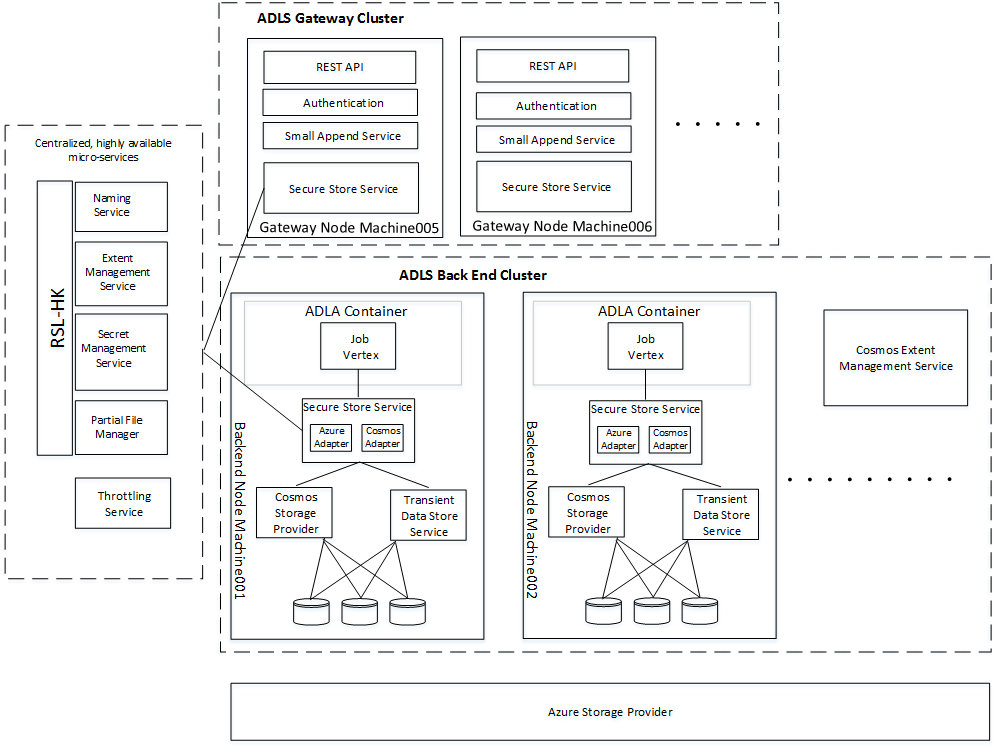
\includegraphics[width=0.84\linewidth]{figs/ADLS-arc.png}
	\caption{架构图(\cite{ramakrishnan2017azure}图2-2)}%TODO
	\label{fig:ADLS-arc}
\end{figure}

ADLS主要支持五种基本的文件操作,open、append、read、concatenation、enumeration。这些操作基于ADLS独特的文件系统设计(partial file和extent),有些操作会变得异常高效:如append只用取一个extents来进行修改,减少了大文件的I/O;concatenation 甚至不用文件I/O,只用在NS和PFM中做修改。具体的操作流程如下:\\
\textbf{open:} 
\begin{itemize}
	\item 创建一个文件:Secure Store Service(SSS)在Naming Service(NS)中创建一个索引。SSS选择一个 storage provider (如Azure Storage)存储tail partial file,并在Partial File Manager(PFM)中创建一个索引。SSS请求存储提供商创建一个文件索引。
	\item 打开一个文件:SSS在NS索引中搜索文件得到File ID。SSS在PFM索引中搜索File ID得到Provider ID和tailed partial file ID
\end{itemize}
\textbf{append:}
\begin{itemize}
	\item fixed-offset append:用户确定数据在文件中的偏移,如果文件中该偏移下有数据,操作异常中止。
	\item free offset append:ADLS自动设置文件偏移,加在文件末尾。
\end{itemize}
\textbf{read:}
\begin{itemize}
	\item Specifying a byte range to read:数据可能同时在多个storage provider上存储,SSS选择最快的读。
	\item Access extents directly:先得到文件的元数据,然后通过元数据去寻找对应的extent
\end{itemize}
\textbf{concatenation:}把多个文件连成一个文件。只需要修改NS和PFM中的索引即可。\\
\textbf{enumeration:}返回文件长度和最近修改时间。如果文件是sealed,那么只用访问PFM就行。如果文件是unsealed,SSS会询问存储tailed partial file的storage provider。

\newpage
\section{一个简单的Serverless平台原型(汪润川)}
\subsection{简述}
为了对 Serverless 计算有一个比较直观的认识,我们调研了一个供研究和测试用的 Serverless 平台原型\cite{mcgrath2017serverless}。该平台原型由 .NET 实现,部署在 Microsoft Azure 上,以 Windows 容器为函数执行环境。其基本架构如图\ref{figs:mcgrath2017_structure}所示,包括 Web 和 Worker 两个服务,中间消息层,以及代码和元数据存储平台。消息层和存储平台依赖 Azure Storage 实现。Web 服务暴露平台的公共 REST API,接收外部的调用消息,实现前后端的交互;一个 Worker 服务管理若干容器。
\begin{figure}[!htbp]
	\centering
	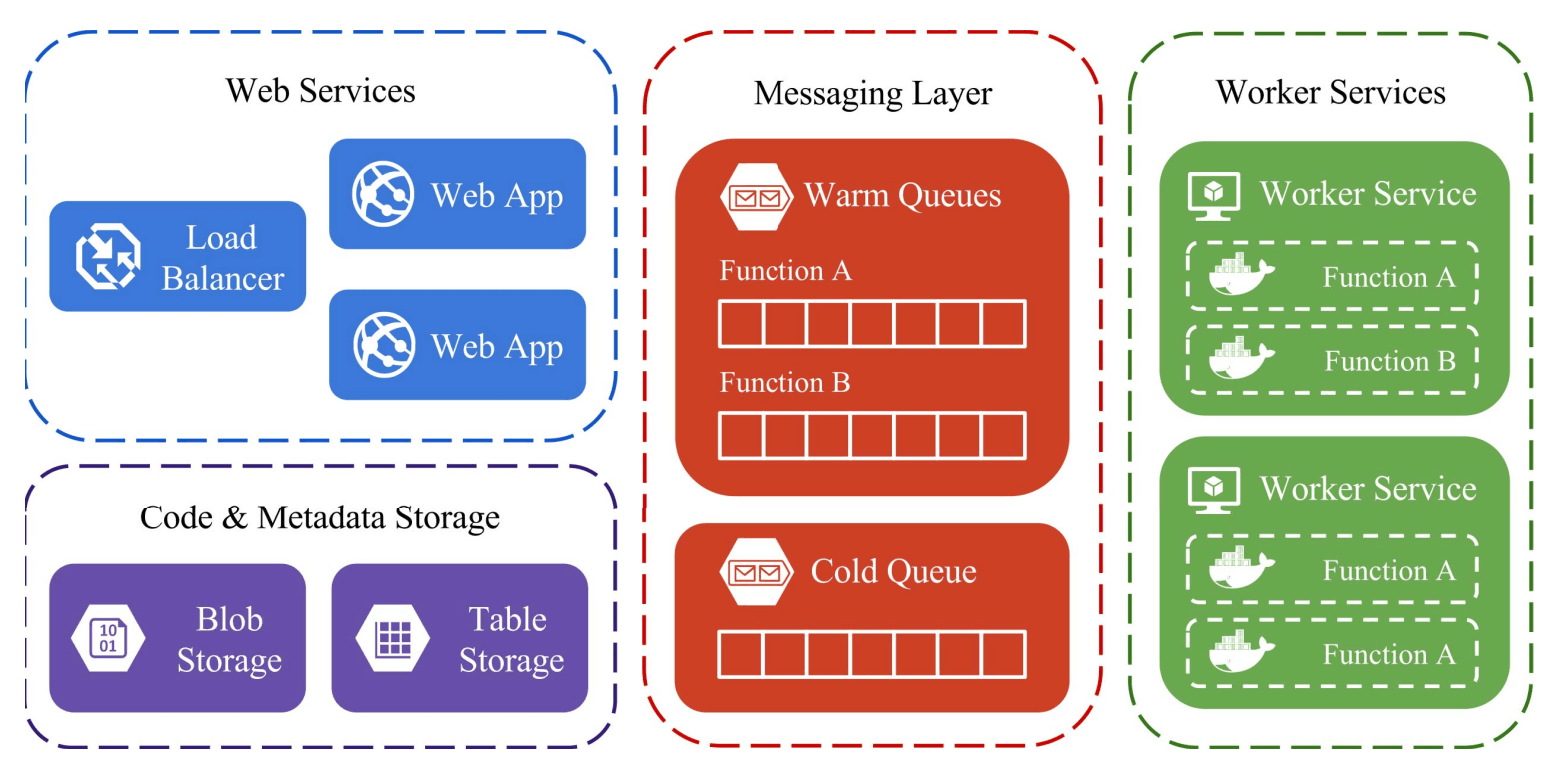
\includegraphics[width=0.9\linewidth]{figs/2017serverless_structure}
	\caption{Serverless 平台原型的基本架构。(\cite{mcgrath2017serverless}图1)}
	\label{figs:mcgrath2017_structure}
\end{figure}

\subsection{设计结构}
\subsubsection{函数元数据}
函数元数据(Function Metadata)是函数在执行过程中必须依赖的数据, 由四个部分构成:
\begin{enumerate}
	\item 函数标识符:全局唯一标识符(GUID),在函数创建时随机产生,用于唯一识别函数和函数资源。
	\item 语言运行时:规定了编写函数的语言。原型目前只支持 Node.js。
	\item 内存大小:决定了函数在容器内可以使用的最大内存容量。上限为 1 GB。
	\item 代码 Blob URI:函数的代码打包存储于云端平台,函数元数据记录 blob URI。
\end{enumerate}

\subsubsection{函数执行}
原型提供一个基本的函数执行模型,仅仅支持手动调用。当一个调用到达时,Web 服务首先接收调用信息(包括函数的输入),并从云端存储中获得函数元数据。输入和元数据共同构成函数的执行请求。Web 服务会尝试寻找 Worker 服务里可用的容器并提交执行请求。如果 Web 服务成功获得一个可用的容器, Worker 服务将执行函数并返回结果。


Web 服务和 Worker 服务之间通过一个共享的消息层进行联系。消息层中有两种队列:对所有函数一致的冷队列和每个函数独有的暖队列。队列中存储容器信息,包括 Worker 实例的地址以及容器名。冷队列中的容器没有被分配内存,使用时需要被启动。暖队列中的容器已经被分配内存,如果从队列中取到的容器刚好是空闲的,那么函数可直接使用。


Web 服务首先尝试从暖队列中获取一个空闲容器,如果不成功(可能暖队列为空,或者暖队列的首个容器正在被使用),则再从冷队列中获得一个容器,在 Worker 上部署和启动这个新容器。如果 Worker 的所有内存资源都被分配出去,那么冷队列为空。此时, Web 服务将无法在两个队列中获得可用的容器,会返回一个 HTTP 例外。冷队列反映了计算平台可用空间的多少,可以支持自动伸缩特性。

\subsubsection{容器分配}
每一个 Worker 管理自己的空闲内存池。若空闲的内存(既没有被分配也没有被预留的内存)大于函数可用的最大内存(1GB)时,这块大小为 1GB 的内存就会被预留。Worker 会为这块内存生成一个独有的容器名。此时,这块内存仅仅是被预留而非分配给容器和函数,因此内存信息和容器名会作为一个消息放入冷队列中。当一个冷队列中的容器需要被启动时,Worker 会根据函数元数据规定的内存大小真正的给容器分配内存,这时,这个容器的信息就由冷队列首转移到了暖队列尾。

\subsubsection{容器移除}
有两种情况容器会被移除。第一种情况是函数被删除,从而 Web 服务删除了函数的暖队列,Worker 则会定期监测暖队列的存在。第二种情况是容器被闲置超过15分钟。这两种情况下,Worker 会删除原函数所使用的容器并回收内存。回收的内存是空闲内存,当空闲内存超过函数可用的最大内存(1 GB)时,系统会预留容器,并向冷队列发送这个容器的消息。如果容器因函数闲置而被删除,当函数被再次调用时, Worker 服务会向函数返回 HTTP 例外,函数此时只能重新申请启动一个冷队列中的容器。

\subsubsection{容器镜像}
平台采用 Docker 运行容器,容器镜像包括函数运行时(目前只支持 Node.js)以及执行处理程序,而不包括任何函数代码。容器启动时,由平台在容器内附一个只读的函数代码,容器的可使用的内存资源也根据函数需要的内存大小进行分配。这样操作可以不用为每一个函数单独创建一个镜像,简单快捷。


容器的执行处理程序是一个简单的 Node.js 服务,它通过 HTTP 请求从 Worker 服务获取函数的输入,并给 Worker 返回函数的结果。

\subsection{评测结果}
作者将他设计的 Serverless 原型和市场上的主流 Serverless 计算平台进行了比较,包括 AWS Lambda, Azure Functions, Google Cloud Functions, Apache OpenWhisk。作者设计了两种测试方法:并发测试和退避测试。


并发测试评价系统的并发函数调用能力。测试工具在收到上一次函数的执行结果后,立即提交新的函数执行请求。测试开始时,一次只提交一个函数执行请求。每隔10秒增加一个并行函数,最多测试15个函数并行执行的效果。评测按照每秒收到的响应作为指标,评测结果如图\ref{figs:2017_concuttent_test}。
\begin{figure}[!htbp]
	\begin{subfigure}[b]{0.43\linewidth}
		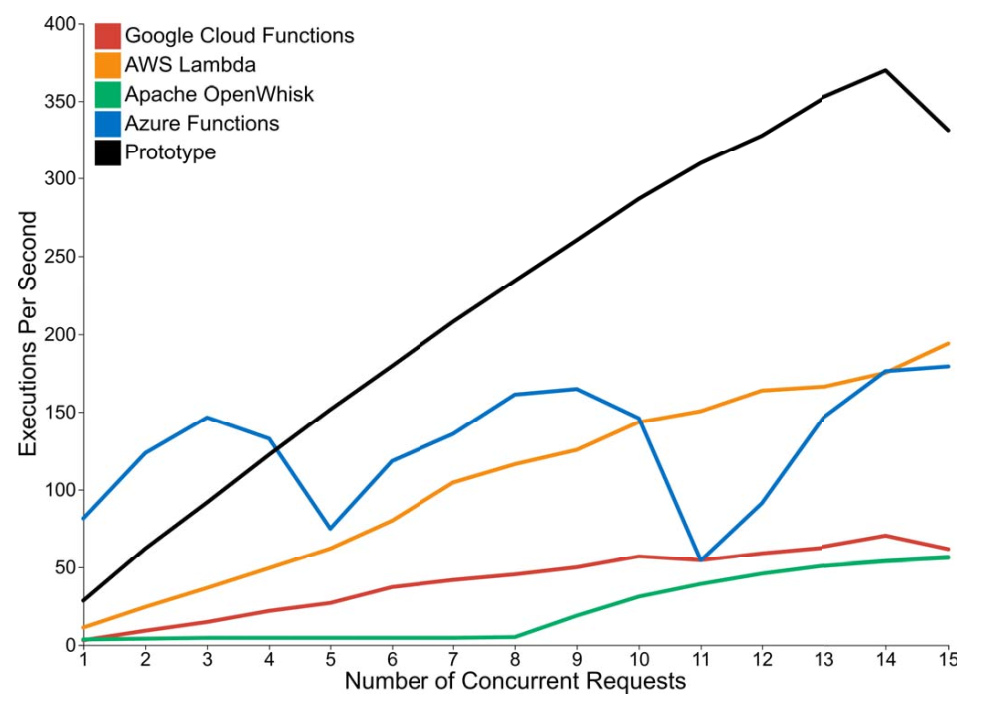
\includegraphics[width=\linewidth]{figs/2017_concuttent_test}
		\caption{}
		\label{figs:2017_concuttent_test}	
	\end{subfigure}
	\begin{subfigure}[b]{0.57\linewidth}
		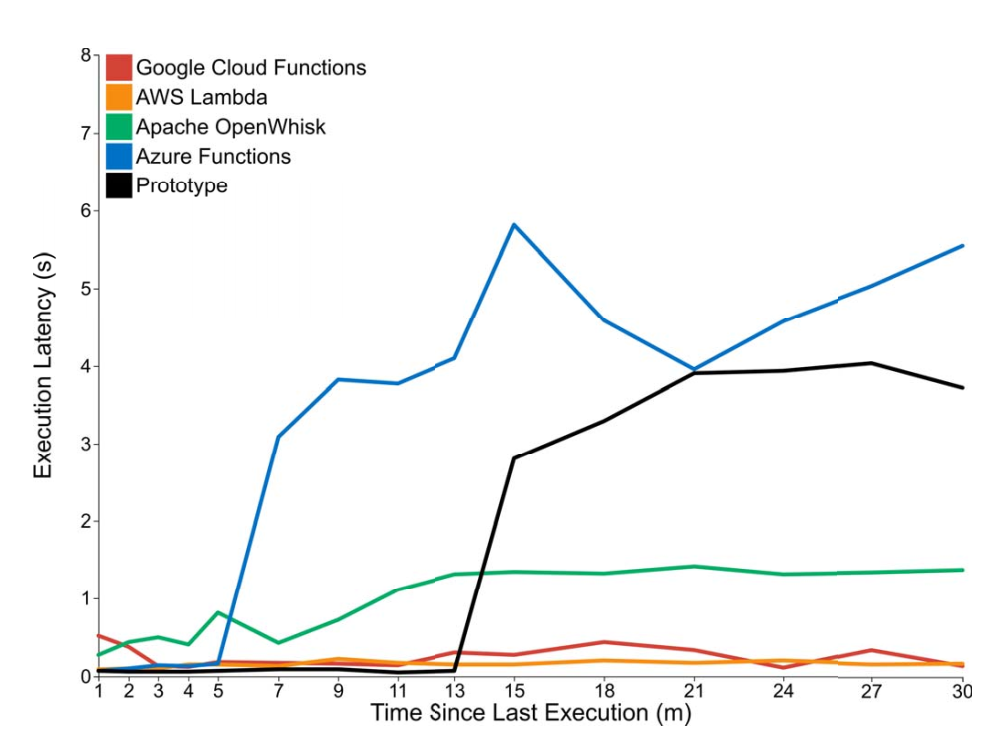
\includegraphics[width=0.8\linewidth]{figs/2017_backoff_test}
		\caption{}
		\label{figs:2017_backoff_test}
	\end{subfigure}
	\caption{(a) 并发测试结果。(b) 退避测试结果。(\cite{mcgrath2017serverless}图2、3)}
\end{figure}

在作者的平台上,如果并发函数小于15个,每秒执行次数与函数数量呈线性关系,但并发数为15时每秒执行次数下降。原因在于此时的负载已经接近单个 Azure 队列的伸缩极限,从而造成暖队列的延迟。其他的商用平台,AWS Lambda 的每秒执行数与函数数量呈线性关系,且有最高的吞吐量。 Google Cloud Functions 呈亚线性关系,并在15个并发函数处性能下降。 Azure Functions 呈波动关系。 OpenWhisk 在8个以下的并发函数都呈现低吞吐量,8个以上函数后呈亚线性关系,这可能是因为 OpenWhisk 的容器池会首选开启新的容器,而不是重新利用已开启的容器。

退避测试用于评价 Serverless 平台应对冷启动以及函数终止的表现。测试会按照递增的时间间隔向测试函数发送单个执行请求,时间间隔由1分钟向30分钟递增。测试结果如图\ref{figs:2017_backoff_test}。


再作者的平台上,根据设计,如果容器被闲置15分钟,那么它将会被收回,在这之后执行函数会遇到冷启动的问题。实验结果也反映出来,在15分钟后,原型的延迟会变得很高。Azure Functions 同样有着明显的冷启动问题。OpenWhisk 在10分钟之后会有轻微的冷启动问题,但和原型以及 Azure Functions 相比并不明显。Google Cloud Functions 和 AWS Lambda 几乎没有冷启动问题,可能是因为它们的容器启动时间短,或者容器在启动前有一个预分配内存的过程。

\subsection{讨论}
该 Serverless 原型还有如下的问题和可以改进的地方:
\begin{enumerate}
	\item 暖队列。已分配内存的容器放在队列中,会导致空闲容器堵塞的问题。一个容器即使执行完毕,如果在它之前分配的容器还没有执行完毕,那么这个容器并不能被 Web 看到并且使用。它必须等待之前分配的容器完成执行,或者自己闲置 15 分钟后被回收。这类问题需要栈或持续性哈希等结构的配合进行解决,然而 Azure 存储平台暂不支持这些数据结构。
	\item 异步执行。当前的平台只支持同步执行,即一个执行请求在提交之后必须等待函数执行完成,返回执行结果。异步执行允许执行请求只调用函数,不需要等待函数结果。异步执行的难点在于要保证至少一次执行。可以采用队列记录执行的函数,并增加一个监控服务,检测因平台问题而执行失败的函数,并重新执行。
	\item Worker 利用率。实际应用中, Worker 的资源通常会被过度分配,因为并非所有的函数都会持续执行,或是完全利用内存空间,这就涉及到执行效果和计算开销上的平衡。这个问题需要对大量的执行负载进行分析。
	\item Windows 容器。Windows 容器相比于 Linux 容器有着很大的不足。在平台原型中,Windows 容器无法在闲置的时候暂停,只能关闭和回收。另外,Windows 容器的可用资源必须在函数执行前配置好,无法在执行请求到达时再进行动态调整。
	\item 安全性。虽然容器已经被精心设计,函数权限也有限制,但将用户的所有代码托管在容器中依然是非常危险的行为。未来仍需要对函数执行环境的被攻击可能性进行评估。
	\item 测试方法。还有更多可以测试的内容,比如不同语言进行时的延迟比较、代码大小的延迟比较、系统事件类型比较、CPU 分配比例等等。
\end{enumerate}

作者的 Serverless 平台虽然比较简单,支持的功能也有限,但已经具有了一般 Serverless 平台的特点,包括函数驱动,自动部署,自动扩容缩容等。其遇到的问题,如冷启动,也是 Serverless 商用平台所需要解决的。

\section{Knative与Google Cloud Run(汪润川)}

\subsection{简述}
传统的 Serverless 存在着厂商绑定、缺乏行业标准的问题,为此,Google 联合 Redhat, IBM 等公司推出了 Knative 框架,旨在提供一套简单易用的 Serverless 计算方案,把 Serverless 标准化。它以分布式容器 Kubernetes 为基础,并提供了缩容到零、自动扩缩、集群内构建以及事件框架等功能。Knative 于2018年7月推出,目前仍在快速发展阶段。Google Cloud Run 是 Knative 的完全托管版本。

\begin{figure}[!htbp]
	\centering
	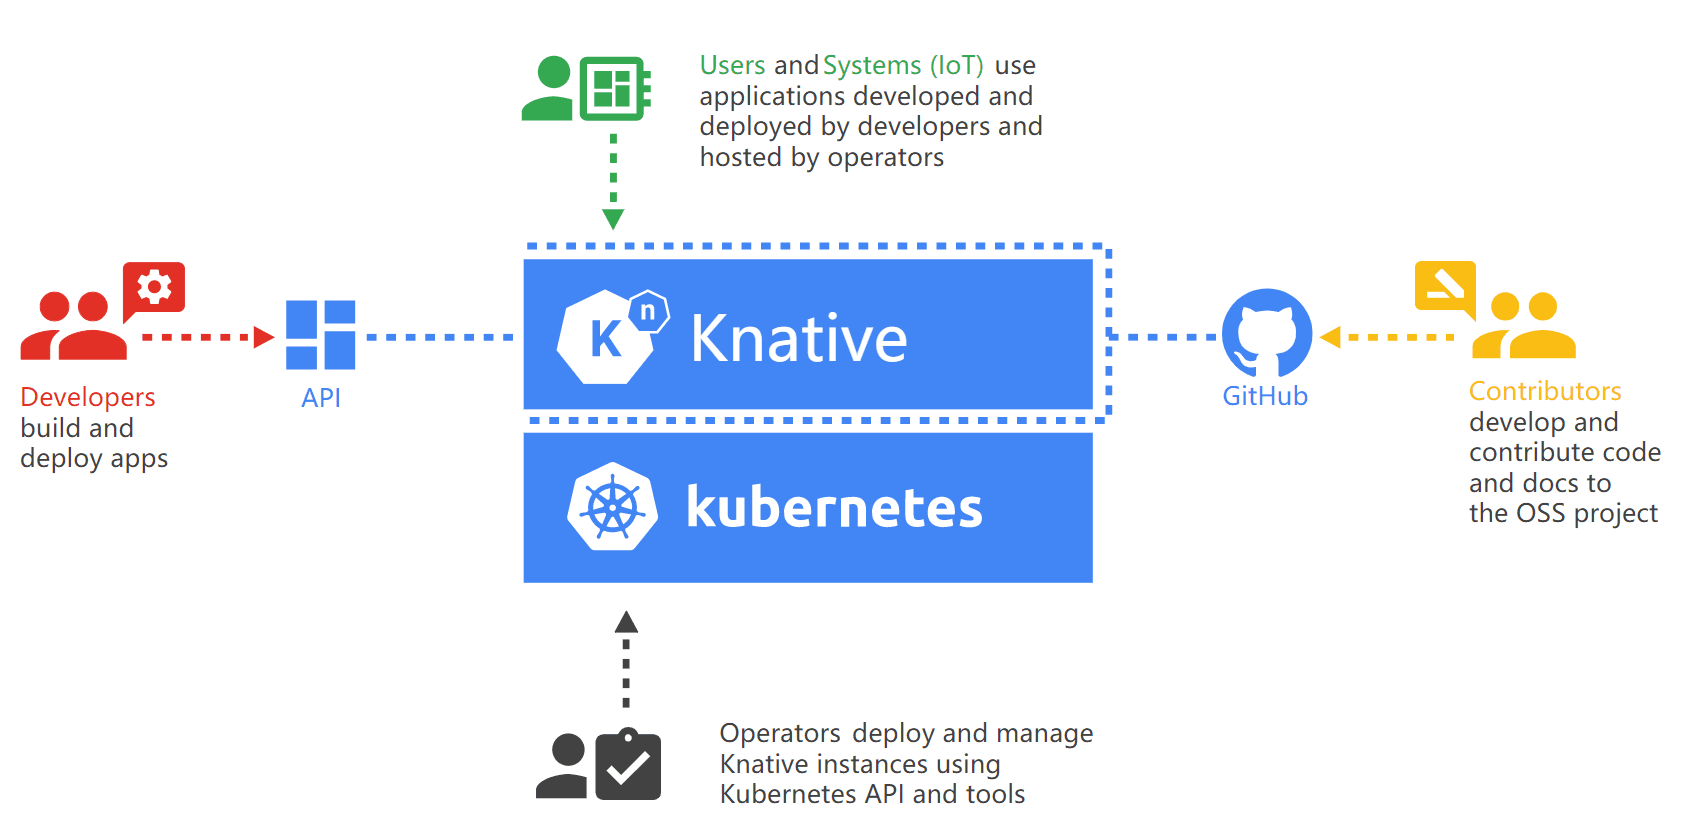
\includegraphics[width=1.0\linewidth]{figs/knative-audience}
	\caption{Knative 是基于 Kubernetes 的 Serverless 扩展。(\cite{knative-audiance})}
	\label{figs:knative-audience}
\end{figure}


Kubernetes(k8s)是自动化容器操作的开源平台,这些操作包括部署,调度和节点集群间扩展。Kubernetes 支持 Docker,Rocket 等容器技术。 Kubernetes 本身非常强大,但它十分复杂,开发人员需要理解并管理其丰富的资源,以及学习很多相关工具(yaml, kubectl, Istio, ...)。 Kubernetes 的理念与云原生(Cloud Native)背道而驰。Knative 是一个 Serverless 版的 Kubernetes ,使得开发人员可以只专注于业务代码而非基础设施。当然,如果 Knative 不能满足开发人员的需求,Knative 背后的 Kubernetes 功能依然可以被直接使用。下面简单介绍一些与 Knative 相关的 Kubernetes 概念。


Pod 是 Kubernetes 最小的调度单位,Pod 从属于 Node(物理机或虚拟机),Pod 中可以运行多个 Docker 容器,处于一个 Pod 中的多个容器共享共享网络和文件系统,以及 PID、IPC、Network 和 UTS 的命名空间\cite{k8s-pod}。Pod 在创建时会被分配一个IP地址,Pod 间的容器可以互相通信。Deployment 是 Pod 版本管理的工具,用来区分不同版本的 Pod。ReplicaSet 是副本控制器,使 Pod 副本数量始终维持在预设的个数。


Kubernetes 中的所有事物都被视为一个 API 对象并且都有一个与之对应的 API 入口。所有的操作和组件间的通信,包括外部的用户命令,都是由 API Server 处理的 REST API 调用。在 Kubernetes 中一切都可视为资源,系统提供了很多默认资源类型,如 Pod、Deployment等。一种资源就是 Kubernetes API 中的一个端点,它存储着某种 API 对象的集合。自定义资源(CRD)是对 Kubernetes API 的扩展,在一个运行中的集群内,自定义资源可以通过动态注册出现和消失,集群管理员可以独立于集群本身更新自定义资源\cite{k8s-CRD}。


Knative 包含2个核心组件: Serving 和 Eventing。Serving 提供 Serverless 应用或函数的部署能力以及各种服务管理,底层采用 Kubernetes 的 Pods;Eventing 管理进入到环境中的事件,提供事件触发的通道。事件不仅要被送达到相应的服务,也要被持久化到某些队列中去,以适应目标服务当前不可用的情况。同时,Knative 还依赖于 CI/CD 流水线 Tekton 完成从代码到部署的过程。

\subsection{Knative 组件}
\subsubsection{Tekton} \label{Tekton}
早期 Knative 采用一个专门的 Build 组件将源码构建成容器,Build 组件完全基于 Kubernetes 生态,用 Kubernetes CRD 的方式实现。Build 组件现已不再维护和推荐使用,当前推荐的构建组件是持续集成和持续部署(CI/CD)流水线 Tekton Pipelines。Tekton 以自定义资源的形式提供了一组 Kubernetes 扩展,用于定义流水线。图\ref{figs:knative-TektonPipeline}展示了 Tekton Pipelines 的 CRD\cite{knative-TektonPipeline},包括:
\begin{figure}[!htbp]
	\centering
	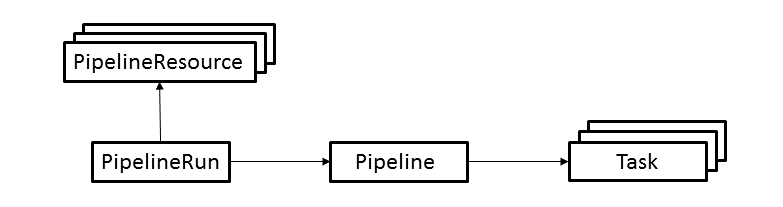
\includegraphics[width=0.8\linewidth]{figs/knative-TektonPipeline}
	\caption{Tekton CRD 结构。(\cite{knative-TektonPipeline})}
	\label{figs:knative-TektonPipeline}
\end{figure}
\begin{itemize}
	\item PipelineResource:定义了一个对象,该对象是流水线的输入(例如 git 存储库)或输出(例如 docker 镜像)。
	\item PipelineRun:定义了流水线的执行。它引用要运行的 Pipeline 以及要用作输入和输出的 PipelineResources。
	\item Pipeline:定义了构成流水线的 Tasks。
	\item Task:定义了一组构建步骤,如编译代码、运行测试以及构建和部署镜像,相当于一系列模板。
\end{itemize}

图\ref{figs:knative-source_to_image}展示了将一个应用从源码构建成容器镜像,然后再部署到 Knative 环境上的过程\cite{knative-source_to_image}。这个过程包括 Build (构建)和 Deploy (部署)两个 Tasks(任务),这两个任务通过一个 Pipeline 封装。 PipelineResource 包括了应用的源码,以及构建和部署会使用到的配置文件。 Build 阶段, kaniko (一款可以进行容器镜像构建的开源工具)会根据 Dockerfile 将源码构建成一个镜像,并上传到 Docker Registry 上。容器构建完成后, Build 会将镜像名、版本等信息传给 Pipeline 下游的任务。第二个任务同样从 PipelineResource 中获取部署的文件,利用 kuberctl (Kubernetes 的命令行工具)将 Docker Registry 上的镜像完成部署。

\begin{figure}[!htbp]
	\centering
	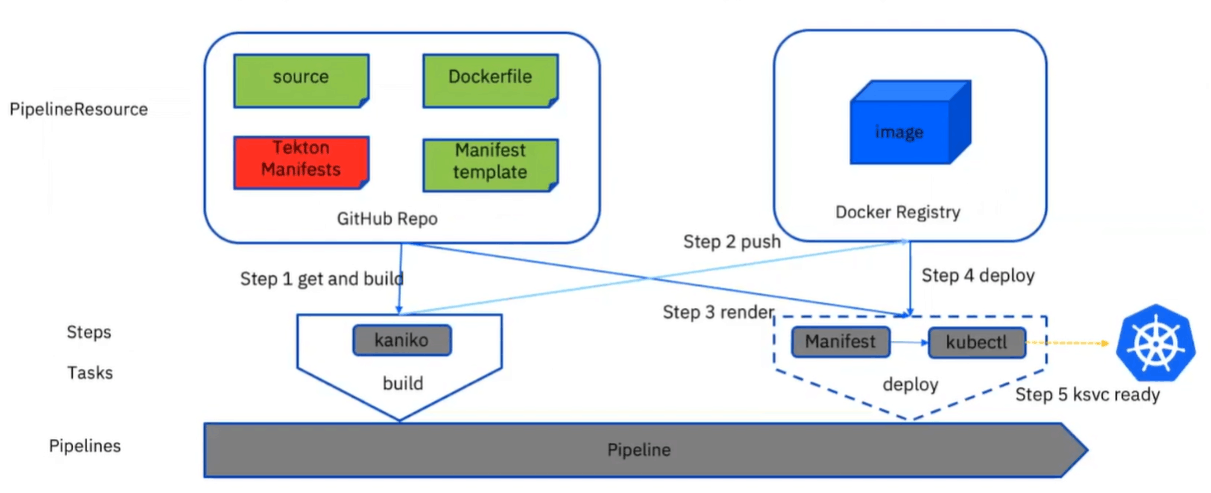
\includegraphics[width=1.0\linewidth]{figs/knative-source_to_image}
	\caption{利用 Tekton 从源码构建容器镜像。(\cite{knative-source_to_image}Page.12)}
	\label{figs:knative-source_to_image}
\end{figure}

\subsubsection{Serving}
Serving 提供了 Serverless 应用或函数的部署能力,以及自动缩扩容、版本管理、流量控制、滚动升级等功能。Serving 的基本结构如图\ref{knative-serving}所示,它提供四个主要的 API\cite{knative-servingapi}:
\begin{itemize}
	\item Route: 定义网络端口,映射一个或多个 Revision,将流量按比例导入不同的 Revision。
	\item Revision: 应用的旧版本,每次修改代码或配置的快照,可以根据进入的流量自动扩缩容。
	\item Configuration: 维护应用的最新配置,每次修改 Configuration 会产生一个新的 Revision。
	\item Service: 管理应用的整个生命周期,确保应用拥有 Configuration 和 Route。Service 可以被看作是正在部署的应用或者函数。
\end{itemize}
当需要进行滚动升级时,Route 会将所有流量逐渐路由到最新的版本中,而旧版本最终会因为没有流量而缩容至0。

\begin{figure}[!htbp]
	\begin{subfigure}[b]{0.48\linewidth}
		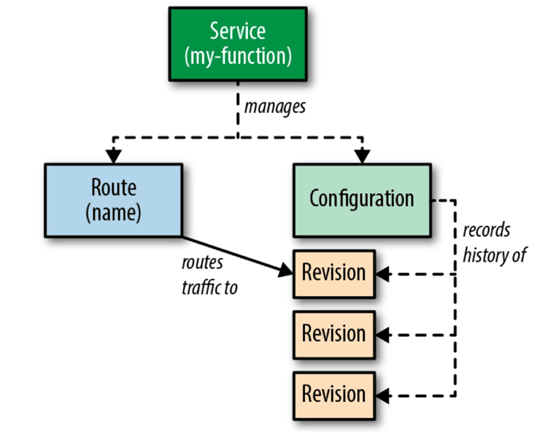
\includegraphics[width=\linewidth]{figs/knative-serving.png}
		\caption{}
		\label{knative-serving}
	\end{subfigure}
	\begin{subfigure}[b]{0.52\linewidth}
		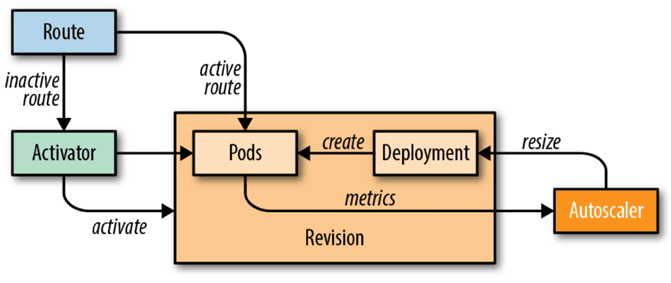
\includegraphics[width=\linewidth]{figs/knative-autoscaler.png}
		\caption{}
		\label{knative-autoscaler}
	\end{subfigure}
	\caption{(a) Serving 基本结构。(b) Autoscaler 实现自动缩容扩容。(\cite{mcclain2019getting}图2-1、2-2)}
\end{figure}

Revision 的自动缩容扩容功能还需要 Autoscaler 和 Activator 两个组件完成\cite{mcclain2019getting}。Reversion中的Pod会自动汇报metrics数据到 Autoscaler,Autoscaler 会根据请求量和资源使用情况修改Deployment的副本(replicas)数量,从而实现自动扩缩容。

Revision 处于激活状态才接受请求。当一个 Revision 停止接受请求时,Autoscaler将其置为待命状态。处于待命状态下,一个 Revision 底层部署缩容至零并且所有到它的流量均路由至 Activator。Activator 是一个共享组件,捕获所有到待命 Revision 的流量。当它收到某一待命 Revision 的激活请求后,它转变 Revision 状态至激活,然后代理请求至合适的 Pod。

\subsubsection{Eventing}
Knative Eventing 是一个旨在满足云原生开发的常见需求的事件平台,提供可组合的元素以支持后期绑定事件生产者和事件消费者。特征是松耦合、事件生产者和消费者互相独立、支持第三方服务接入、支持跨平台和互操作性\cite{knative-eventing}。


Eventing 定义了一组 Kubernetes CRD,包括
\begin{itemize}
	\item Event Source: 用于把事件生产者接入 Knative 事件平台,并把事件传送给消费者。
	\item Channel: 实现事件的转发和存储。底层实现可以有 Kafka, NATS Streaming 等。
	\item Subscription: 事件的订阅者,即事件转发的目的地。
	\item Parallel: 事件同时转发给多个订阅者,每个订阅者接收到同一个事件。
	\item Sequence: 事件依次经过多个订阅者,每个订阅者都可以修改,过滤或者创建新的事件。
	\item Broker: 可以接收事件,并将事件根据过滤条件转发给订阅者。
	\item Trigger: 根据订阅者的要求对事件设置过滤条件过滤。
	\item Event Registry: 用于查阅 Broker 中的事件类型。
\end{itemize}

Sink 是 Eventing 中一个重要概念,表示事件消息传送的目的地,也就是事件接收者的一个 HTTP 端口。


一个简单的事件订阅流程如图\ref{knative-cha_sub}所示。 Event Source 定义了事件源,通过 Sink 指定事件消费者的地址。 Knative 规定传输的事件必须符合 CloudEvents 格式,因此在 Event Source 后还有一个 Adapter(图中未画出)进行格式转换。为了适应单个事件源对多个订阅者的场景,需要使用 Channel 和 Subscription。 Channel 具有存储功能,可以避免消费者因暂时不在线而导致的消息丢失。 Subscription 连接 Channel 和消费者。消费者可以通过 Subscription 接收消息,也可以向 Subscription 发送回复,并由 Subscription 向其他 Channel 转发。基于 Channel 和 Subscription ,可以实现 Parallel 和 Sequence。
\begin{figure}[!htbp]
	\centering
	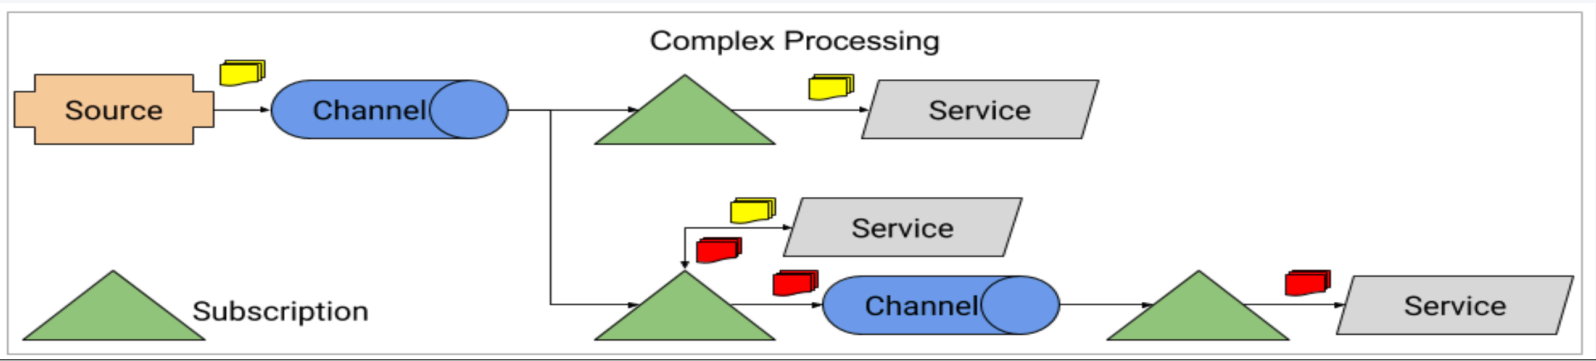
\includegraphics[width=\textwidth]{figs/knative-cha_sub.png}
	\caption{通过 Channel 和 Subscription 实现事件的转发和订阅。(\cite{knative-eventing}Page.18)}
	\label{knative-cha_sub}
\end{figure}

在较新的 Knative 版本中,Eventing 增加了 Broker 和 Trigger 对象,目的是搭建一个黑盒,将具体的实现隐藏起来,减少需要用户添加的 Channel 和 Subscription。同时, Broker 和 Trigger 可以满足消费者对信息过滤的需求,消费者可以选择订阅自己感兴趣的事件,而非接收 Channel 中的所有信息。Eventing 支持的过滤指标包括事件类型和来源,以及任何其他的事件属性。

\begin{figure}[!htbp]
	\centering
	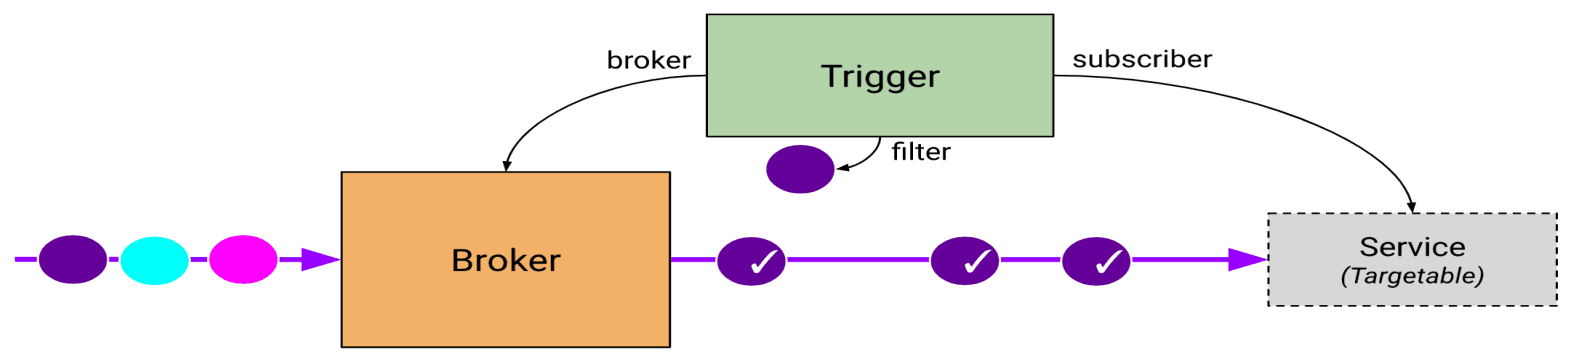
\includegraphics[width=\textwidth]{figs/knative-broker_2.png}
	\caption{通过 Broker 和 Trigger 实现事件的转发和订阅。订阅者告诉 Trigger 只要紫色的消息。Broker 对消息进行过滤,将紫色的消息发送给订阅者。(\cite{knative-eventing}Page.23)}
	\label{knative-broker}
\end{figure}
消费者此时不需要创建 Subscription 对象,而是创建一个 Trigger 对象,描述自己感兴趣的事件。Broker 是一个事件桶,接收各种事件,根据 Trigger 中定义的规则,对事件进行过滤,过滤之后发送给事件的订阅方。事件的转发和订阅结构如图\ref{knative-broker}所示。

\subsubsection{gVisor}
gVisor 是 Google 发布的沙箱技术,用于安全隔离宿主机和应用程序,提供比容器更为安全的隔离机制。gVisor 可以与 Docker 和 Kubernetes 集成在一起。Knative 的容器实际运行于与 Kubernetes 集成的 gVisor 上。在 Kubernetes 中,大多数资源隔离以 Pod 位单位,因此 Pod 也是 gVisor 沙箱的边界\cite{knative-gvisor}。gVisor为 Cloud Run 带来了安全容器的隔离,但是也带来了一些限制,例如,gVisor 支持的系统调用是有限的\cite{cloudrun_contract}。
\begin{figure}[!htbp]
	\centering
	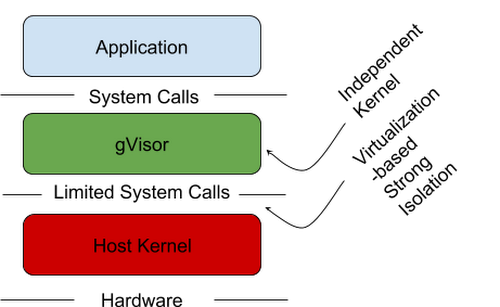
\includegraphics[width=0.7\textwidth]{figs/knative-gvisor.png}
	\caption{gVisor 支持的系统调用是有限的。(\cite{knative-gvisor}图3)}
	\label{knative-gvisor}
\end{figure}

\subsection{实际操作:构建和部署}
在这一节中,我们将根据 Google Cloud Run 文档中的教程\cite{cloudrun}构建和部署一个简单的 Hello-World python 应用,从程序员的视角体验 Knative 给开发带来的便利。Cloud Run 对运行的容器有如下要求和限制\cite{cloudrun_contract}:
\begin{itemize}
	\item 容器必须是 64 位 Linux 平台。
	\item 在 8080 端口监听 HTTP 请求。
	\item 容器必须在收到请求 4 分钟之内启动 HTTP 服务器。
	\item 每个容器默认可使用 256 MB 内存,最多可以使用 2GB 内存。
\end{itemize}

下面开始准备工作,首先注册 \href{https://cloud.google.com/}{Google Cloud} 账号。注册时需要提供信用卡信息,首次注册可以获得1年的免费使用期和 300 美元赠金。注册成功后打开 \href{https://console.cloud.google.com/}{Google Cloud 控制台},点击上方选择项目按钮,在弹出的对话框中选择“新建项目”,给新项目命名(如图\ref{figs:name}),系统会自动生成一个项目ID。创建项目后,为新创建的 Hello-World 项目启用 Cloud Build API,如图\ref{figs:start}。
\begin{figure}[!htbp]
	\begin{subfigure}[b]{0.5\linewidth}
		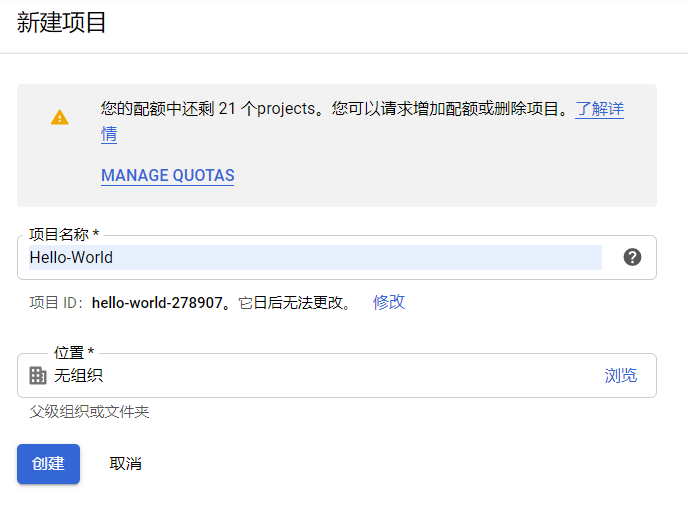
\includegraphics[width=\linewidth]{figs/cloudrun_name.png}
		\caption{}
		\label{figs:name}
	\end{subfigure}
	\begin{subfigure}[b]{0.5\linewidth}
		\includegraphics[width=\linewidth]{figs/cloudrunstartapi.png}
		\caption{}
		\label{figs:start}
	\end{subfigure}
	\caption{(a) 创建新的项目。(b) 启动 Cloud Build API。}
\end{figure}

在本地机器上安装和初始化 \href{https://cloud.google.com/sdk/docs}{Google Cloud SDK} \footnote{即使开了网络代理,Cloud SDK 在中国大陆地区的初始化也会遇到网络连接失败的问题。虽然可以在 Cloud SDK 中再配置代理信息,但为了方便起见,我直接在海外服务器上安装 Cloud SDK。因此,海外服务器是我开发的本地环境。}。Cloud SDK 是 Google Cloud 的命令行工具,用于访问 Google Cloud 的相关资源。Linux 系统下,Cloud SDK 的安装依赖于 Python 3。运行初始化 Cloud SDK 的命令
\begin{lstlisting}
# gcloud init
\end{lstlisting}
初始化阶段需要登录 Google Cloud 账号以及选择默认的项目。
在本地环境中编写应用代码:
\lstinputlisting[
%style = Python,
caption = {app.py}
]{./code/app.py}

此代码使用“Hello Bigdata”响应请求,以8080为监控端口。根据\ref{Tekton}节的部署要求,我们还需要创建一个 Dockerfile 作为容器的配置信息:
\lstinputlisting[
%style = Python,
caption = {Dockerfile}
]{./code/Dockerfile}

添加一个 .dockerignore 文件,以从容器映像中排除文件:
\lstinputlisting[
%style = Python,
caption = {.dockerignore}
]{./code/.dockerignore}

\begin{figure}[!htbp]
	\centering
	\includegraphics[width=0.8\textwidth]{figs/cloudrun_submit.png}
	\caption{代码和配置信息已被上传。}
	\label{cloudrun_submit.png}
\end{figure}
\begin{figure}[!htbp]
	\centering
	\includegraphics[width=0.8\textwidth]{figs/cloudrun_complete.png}
	\caption{Cloud 控制台可以监控服务的请求数、延迟时间、收费容器实例时间、容器的 CPU 和内存利用率。也可查看服务的版本、日志、权限等信息。}
	\label{cloudrun_complete.png}
\end{figure}

将这三份代码放在一个目录下,在这个目录下执行命令:
\begin{lstlisting}
# gcloud builds submit --tag gcr.io/hello-world-278907/helloworld
\end{lstlisting}
将代码和配置文件上传到 Container Registry 上并构建容器。其中,hello-world-278907 是项目 ID。通过 Google Cloud 控制台,可以看到代码和配置信息已被上传,如图\ref{cloudrun_submit.png}所示。

执行部署命令:
\begin{lstlisting}
# gcloud run deploy --image gcr.io/hello-world-278907/helloworld --platform managed
\end{lstlisting}
输入服务名称,选择部署服务器的位置。等待部署完成,命令行会显示服务网址。我部署的这个服务网址为\url{https://helloworld-wacroj5uba-de.a.run.app/},通过浏览器访问该地址,可以看到“Hello Bigdata!”的问候语。通过控制台,可以监控服务的各项指标,如图\ref{cloudrun_complete.png}所示。

在这个创建和部署的整个过程中,我们只写了应用代码和容器的配置信息,创建和部署只需要一条命令即可执行,非常方便快捷。

\newpage
\section{Microsoft Azure Functions(刘力玮)}
\subsection{基本原理}
Azure Functions是微软推出的一种无服务器计算服务,使用它可以运行事件触发的代码,而无需显式预配或管理基础结构。Azure Functions允许使用者运行小段代码(称为“函数”)且不需要担心应用程序基础结构。借助Azure Functions,云基础结构可以提供应用程序保持规模化运行所需的所有最新状态的服务器。函数由特定类型的事件“触发”。支持的触发器包括对数据更改做出响应,对消息做出响应,按计划运行,或者生成HTTP请求的结果。虽然使用者始终可以直接针对大量服务编写代码,但使用绑定可以简化与其他服务的集成。使用绑定,使用者能够以声明方式访问各种Azure服务和第三方服务。

触发器是导致函数运行的因素。触发器定义函数的调用方式,一个函数必须刚好有一个触发器。触发器具有关联的数据,这些数据通常作为函数的有效负载提供。

绑定到函数是以声明方式将另一个资源连接到该函数的一种方式;绑定可以输入绑定和输出绑定的形式进行连接。绑定中的数据作为参数提供给函数。可根据需要,混合搭配不同的绑定。绑定是可选的,一个函数可以有一个或多个输入绑定和输出绑定。图\ref{fig1}是触发器与绑定的简单实例。

\begin{figure}[!htbp]
	\centering
	\includegraphics[scale=0.6]{figs/1.png}
	\caption{触发器与绑定实例}
	\label{fig1}	
\end{figure}

\subsection{用户手册}
下文介绍使用Visual Studio利用Azure Function开发C\#类库函数并将其发布到 Azure的技术文档。

\subsubsection{必备条件} 
从Visual Studio 2017开始,Azure Functions Tools包含在Visual Studio的Azure开发工作负荷中。确保在Visual Studio安装中包括Azure开发工作负荷并更新为最新版本,如图\ref{fig2}所示。
\begin{figure}[!htbp]	
	\centering
	\includegraphics[scale=0.6]{figs/2.png}
	\caption{Azure开发工作负荷版本更新界面}
	\label{fig2}	
\end{figure}

\subsubsection{创建Azure Functions项目} 
Visual Studio中的Azure Functions项目模板创建一个项目,该项目可发布到Azure中的函数应用。可使用函数应用将函数分组为逻辑单元,以便更轻松地管理、部署、缩放和共享资源。
\begin{enumerate}
	\item 在Visual Studio菜单中,选择“文件” > “新建” > “项目” 。
	\item 在“创建新项目”中,在搜索框中输入“functions”,选择“Azure Functions” 模板,然后选择“下一步”。
	\item 在“配置新项目”中,输入项目的“项目名称”,然后选择“创建”。函数应用名称必须像C\#命名空间一样有效,因此请勿使用下划线、连字符或任何其他的非字母数字字符。
	\item 本例中,对于“创建新的Azure Functions应用程序”设置,使用图3中的设置,确保将“访问权限”设置为“匿名”。如果选择默认级别的函数,需要在请求中提供函数密钥才能访问函数终结点。
	\item 选择“创建”以创建函数项目和HTTP触发器函数,如图图\ref{fig3}所示。
\end{enumerate}
\begin{figure}[!htbp]
	\begin{subfigure}[b]{0.5\linewidth}
		\includegraphics[width=\linewidth]{figs/3.png}
		\caption{}
		\label{fig3}
	\end{subfigure}
	\begin{subfigure}[b]{0.5\linewidth}
		\includegraphics[width=\linewidth]{figs/4.png}
		\caption{}
		\label{fig4}
	\end{subfigure}
	\caption{(a) 创建新函数。(b) 本地设置文件结构。}
\end{figure}
此项目模板创建C\#项目,安装\texttt{Microsoft.NET.Sdk.Functions NuGet}包,并设置目标框架。新项目包含以下文件:
\begin{itemize}
	\item \texttt{host.json}:用于配置 Functions 主机。在本地和Azure中运行时,都会应用这些设置。 
	\item \texttt{local.settings.json}:维护本地运行函数时使用的设置。在Azure中运行时不使用这些设置。
\end{itemize}

\subsubsection{本地设置文件} 
local.settings.json文件存储应用设置、连接字符串和本地开发工具使用的设置。只有在本地运行项目时,才会使用 local.settings.json 文件中的设置。本地设置文件的结构如图图\ref{fig4}。

\subsubsection{将函数添加到项目} 
在C\#类库函数中,可以通过在代码中应用属性来定义函数使用的绑定。从提供的模板创建函数触发器时,将为你应用触发器属性。	
\begin{figure}[!htbp]
	\begin{subfigure}[b]{0.5\linewidth}
		\includegraphics[width=\linewidth]{figs/5.png}
		\caption{}
		\label{fig5}
	\end{subfigure}
	\begin{subfigure}[b]{0.5\linewidth}
		\includegraphics[width=\linewidth]{figs/6.png}
		\caption{}
		\label{fig6}
	\end{subfigure}
	\caption{(a) 添加到项目。(b) 函数代码。}
\end{figure}
\begin{enumerate}
	\item 在“解决方案资源管理器”中,右键单击项目节点,然后选择“添加” > “新建项”。选择“Azure函数”,输入类的名称,然后单击“添加”,如图图\ref{fig5}所示。
	\item 选择触发器,设置绑定属性,然后单击“创建”。以下示例显示创建队列存储触发的函数时的设置。此触发器示例使用具有名为QueueStorage的键的连接字符串。必须在web.config文件中定义此连接字符串设置。
	\item 检查新添加的类。将会看到一个静态Run方法,它已使用FunctionName属性设置了属性。该属性指示该方法是函数的入口点。图\ref{fig6}中的C\#类表示一个基本的队列存储触发的函数。	
\end{enumerate}
已向提供给入口点方法的每个绑定参数提供了特定于绑定的属性。该属性采用绑定信息作为参数。在上面的示例中,第一个参数应用QueueTrigger属性,表示队列触发的函数。 队列名称和连接字符串设置名称作为参数传递到“QueueTrigger”属性。

\subsubsection{添加绑定} 
使用触发器时,输入和输出绑定是作为绑定属性添加到函数的。
\begin{enumerate}
	\item 确保已为本地开发配置项目。
	\item 为特定绑定添加适当的NuGet扩展包。有关详细信息,请参阅“触发器和绑定”一文中的使用Visual Studio进行本地C\#开发。 特定于绑定的NuGet包要求位于绑定的参考文章中。 例如,可以在事件中心绑定参考文章中找到事件中心触发器的包要求。
	\item 如果有绑定需要的应用设置,请将其添加到本地设置文件中的Values集合。当函数在本地运行时,会使用这些值。当函数在Azure的函数应用中运行时,会使用函数应用设置。
	\item 将适当的绑定属性添加到方法签名。在图\ref{fig7}的示例中,一条队列消息触发了该函数,而输出绑定则创建了一条新的队列消息,在不同的队列中使用了相同的文本。
\end{enumerate}	
\begin{figure}[!htbp]
	\centering
	\includegraphics[scale=0.6]{figs/7.png}
	\caption{绑定实例}
	\label{fig7}	
\end{figure}

\subsubsection{函数测试} 
\begin{enumerate}
	\item Azure Functions Core Tools允许在本地开发计算机上运行Azure Functions项目。
	\item 在运行项目时,可以像测试已部署的函数一样测试代码。
\end{enumerate}	

\subsubsection{发布到Azure} 
从 Visual Studio 发布时,使用以下两种部署方法之一。Web部署:将Windows应用打包并部署到任何IIS服务器。启用了从包运行的Zip部署:建议用于Azure Functions部署。
\begin{figure}[!htbp]
	\begin{subfigure}[b]{0.5\linewidth}
		\includegraphics[width=\linewidth]{figs/8.png}
		\caption{}
		\label{fig8}
	\end{subfigure}
	\begin{subfigure}[b]{0.5\linewidth}
		\includegraphics[width=\linewidth]{figs/9.png}
		\caption{}
		\label{fig9}
	\end{subfigure}
	\begin{subfigure}[b]{\linewidth}
		\centering
		\includegraphics[width=0.6\linewidth]{figs/10.png}
		\caption{}
		\label{fig10}
	\end{subfigure}
	\caption{(a) 发布界面。(b) 应用服务界面。}
\end{figure}
本例中使用以下步骤将项目发布到 Azure 中的函数应用。
\begin{enumerate}
	\item 在“解决方案资源管理器” 中,右键单击该项目并选择“发布” 。
	\item 在“选取发布目标” 中,使用图\ref{fig8}中指定的发布选项。
	\item 选择“创建配置文件”。如果尚未从Visual Studio登录到Azure帐户,选择“登录”。也可以创建免费Azure帐户。
	\item 在“应用服务: 新建”中,使用图\ref{fig9}中指定的值。
	\item 选择“创建” ,使用这些设置在Azure中创建函数应用及其相关的资源,并部署函数项目代码。
	\item 选择“发布”,并且在完成部署后记下“站点URL” 值,这是函数应用在Azure中的地址,如图图\ref{fig10}所示。
\end{enumerate}


\subsubsection{函数应用设置} 
必须将在local.settings.json中添加的任何设置添加到Azure函数应用中。 发布项目时,不会自动上传这些设置。

将所需设置上传到Azure中的函数应用的最简单方法是使用“管理应用程序设置...”链接,如图\ref{fig11}所示。

这会显示用于函数应用的“应用程序设置”对话框,可以在其中添加新应用程序设置或修改现有设置,如图\ref{fig12}所示。
\begin{figure}[!htbp]
	\begin{subfigure}[b]{0.5\linewidth}
		\includegraphics[width=\linewidth]{figs/11.png}
		\caption{}
		\label{fig11}
	\end{subfigure}
	\begin{subfigure}[b]{0.5\linewidth}
		\includegraphics[width=\linewidth]{figs/12.png}
		\caption{}
		\label{fig12}
	\end{subfigure}
	\caption{(a) 函数设置界面。(b) 应用设置。}
\end{figure}

本地表示local.settings.json文件中的设置值,远程是Azure的函数应用中的当前设置。 选择"添加设置"以创建新的应用设置。使用“从本地插入值”链接将设置值复制到“远程”字段。 你选择“确定”后,挂起的更改将写入本地设置文件和函数应用。

\subsubsection{函数监视} 
监视函数执行的建议方法是将函数应用与Azure Application Insights集成。Azure Application Insights可以收集日志、性能和错误数据,自动检测性能异常,并提供强大的分析工具来帮助你诊断问题并了解函数的使用方式。

在Azure门户中创建函数应用时,默认情况下会为你完成此集成。 但在Visual Studio发布期间创建函数应用时,Azure中的函数应用集成未完成。可以通过 Functions 轻松地将Application Insights集成从 Azure门户添加到某个函数应用。
\begin{enumerate}
	\item 在Azure门户中,搜索并选择"function app",然后选择函数应用。
	\item 选择窗口顶部的 "未配置 Application Insights标题"。如果看不到此横幅,则你的应用已启用Application Insights。
	\item 使用图\ref{fig13}中的表中指定的设置创建Application Insights资源。
	\begin{figure}[!htbp]
		\centering
		\includegraphics[scale=0.6]{figs/13.png}
		\caption{资源设置}
		\label{fig13}	
	\end{figure}
	\item 选择“应用”。Application Insights资源在与函数应用相同的资源组和订阅中创建。
\end{enumerate}	

\section{Google Cloud Functions(刘力玮)}
\subsection{基本原理}
Google Cloud Functions是用于构建和连接云端服务的一种无服务器执行环境。借助Cloud Functions,使用者可以编写单一用途的简单函数,并将这些函数关联到云端基础架构和服务发出的事件。当所监控的事件发生时,就会触发使用者的函数。使用者的代码将在完全托管的环境中执行。使用者无需预配任何基础架构,也不必费心管理任何服务器。

\subsection{用户手册}	
下文介绍了如何使用Cloud Console创建和部署用Python编写的Cloud Functions函数。当此函数通过HTTP请求触发时,会如图\ref{fig14}所示输出一条消息:

\begin{figure}[!htbp]
	\centering
	\includegraphics[width=0.7\linewidth]{figs/14.png}
	\caption{函数代码}
	\label{fig14}	
\end{figure}	

\begin{multicols}{2}
\subsubsection{准备工作} 
\begin{enumerate}
	\item 在Cloud Console的项目选择器页面上,选择或创建Cloud项目。
	\item 确保Google Cloud项目已启用结算功能。
	\item 启用Cloud Functions API。
\end{enumerate}

\subsubsection{创建函数} 
\begin{enumerate}
	\item 在Cloud Console中打开Cloud Functions概览页面,如图\ref{fig15}所示。
	\item 选择启用了Cloud Functions的项目。
	\item 点击创建函数。
	\item 指定函数名称。
	\item 在触发器字段中,选择HTTP。
	\item 在源代码字段中,选择内嵌编辑器。
	\item 用运行时下拉列表选择 Python 运行时。
\end{enumerate}
 \begin{figure}[H]
 	\centering
 	\includegraphics[width=\linewidth]{figs/15.png}
 	\caption{创建函数界面}
 	\label{fig15}	
 \end{figure}
\end{multicols}

\subsubsection{函数部署} 
部署的运行方式是将包含函数源代码的归档上传到Google Cloud Storage存储分区。使用者可以从本地机器、GitHub或Bitbucket源代码库(通过Cloud Source Repositories)或直接从Cloud Functions API部署Cloud Functions函数。

本例中按照以下方式:
\begin{enumerate}
	\item 点击图\ref{fig16}页面底部的创建。
	\begin{figure}[!htbp]
		\centering
		\includegraphics[scale=0.6]{figs/16.png}
		\caption{函数部署界面}
		\label{fig16}	
	\end{figure}
	\item 点击创建后,Cloud Console将重定向到Cloud Functions概览页面。
\end{enumerate}	

\subsubsection{函数测试} 
\begin{enumerate}
	\item 显示使用者的函数对应的菜单,然后点击图\ref{fig17}测试函数。
	\begin{figure}[!htbp]
		\centering
		\includegraphics[scale=0.6]{figs/17.png}
		\caption{函数测试界面}
		\label{fig17}	
	\end{figure}
	\item 在测试页面上,点击测试函数。输出屏幕会显示文本 "Hello World!"
	\item 现在更改此消息。在触发事件字段中,输入文本 {"message":"Hello, YOURNAME!"}(将 YOURNAME替换为一个名字),然后点击测试函数。
	
	例如,假设输入的名字是“Rowan”。在输出字段中,会看到消息 Hello, Rowan!。在日志字段中,如果状态码为 200,则表示函数已成功执行,如图\ref{fig18}所示。
	\begin{figure}[!htbp]
		\centering
		\includegraphics[scale=0.6]{figs/18.png}
		\caption{函数测试日志}
		\label{fig18}	
	\end{figure}
\end{enumerate}	

\subsubsection{日志查看} 
Google Stackdriver提供了一套监控工具。Stackdriver Logging可捕获并存储Cloud Functions函数日志,会捕获特殊格式的错误日志,并将其显示在Error Reporting信息中心中。

检查日志以通过日志历史记录了解函数的操作,如图\ref{fig19}所示。
返回Cloud Functions“概览”页面,显示使用者的函数对应的菜单,然后点击查看日志。
此时将显示函数的日志历史记录。
\begin{figure}[!htbp]
	\centering
	\includegraphics[scale=0.6]{figs/19.png}
	\caption{日志查看}
	\label{fig19}	
\end{figure}

%TODO 诸侯纷争???

\bibliographystyle{alpha}
\bibliography{../doc}
\end{document}

